%% ===========================================================================
%%  Mesh Registration from Scan-Derived 3D Data
%%  Internship report — Forschungszentrum Jülich, July–September 2026
%%  Khaoula Jellal
%%
%%  Build:  latexmk -pdf main.tex          (pdfLaTeX)
%%      or  latexmk -lualatex main.tex     (better fonts, if Libertinus present)
%% ===========================================================================
\documentclass[
  10pt,
  twoside,
  open=any,
  numbers=noenddot,
  chapterprefix=false,
  parskip=never
]{scrbook}

\usepackage{style/notebook}
\usepackage{amssymb}
\usepackage{tikz}
\usetikzlibrary{arrows.meta,positioning,calc}
\usepackage{pgfplots}\pgfplotsset{compat=1.16}
\newtcolorbox{algbox}[2][]{enhanced,breakable,colback=white,colframe=rule,boxrule=0.4pt,arc=0pt,
  left=6pt,right=6pt,top=3pt,bottom=3pt,fontupper=\small,
  title={\textbf{Algorithm #2}},coltitle=black,colbacktitle=gray!12,fonttitle=\small,#1}

% == Bibliography ==
% natbib + plain bibtex, deliberately, not biblatex+biber: biber is a
% separate Perl subprocess with real startup cost, and on a throttled
% free-tier compile server that overhead is enough on its own to trip a
% timeout even when everything else compiles quickly. Five references do
% not need biblatex's extra machinery.
\usepackage[numbers,sort&compress]{natbib}
\bibliographystyle{unsrtnat}

% == Metadata ==
\hypersetup{
  pdftitle={Mesh Registration from Scan-Derived 3D Data: Correspondence and Optimization in Articulated Parametric Models},
  pdfauthor={Khaoula Jellal}
}

% ===========================================================================
%  FINDINGS LEDGER — declare every load-bearing result here, once.
%  Cite anywhere with \F{F1}. The ledger table in Chapter 1 builds itself.
%  (Fill in / correct as you consolidate your session notes.)
% ===========================================================================
\DeclareFinding{F1}
  {Surface agreement is not anatomical correctness: a fit can score a lower
   Chamfer distance while its skeleton is worse.}
  {Removing the offset and normal penalties gives $0.45\times$ Chamfer but
   $1.25\times$ joint error, worse in 8 of 11 expert specimens.}
  {Validated}

\DeclareFinding{F2}
  {A rebuilt preprocessing pipeline substantially improves mesh topology, but
   this does not translate into a measurable improvement in the downstream
   surface-fit metric: within the tested pipeline, mesh conditioning alone
   does not explain the observed correspondence failures.}
  {Watertightness 44/44 vs.\ existing pipeline (\S3.3); head-to-head Chamfer
   0.000771 vs.\ 0.000737 with registration held fixed.}
  {Validated}

\DeclareFinding{F3}
  {Regional identity and within-region localisation are distinct
   correspondence problems: supplying the correct anatomical region
   recovers only part of the error.}
  {Regional-identity oracle: leg accuracy $0.867\to0.937$, with substantial
   error remaining inside correctly identified structures.}
  {Validated (synthetic)}

\DeclareFinding{F4}
  {Initialisation sensitivity is anatomically heterogeneous: it strongly
   affects distal recovery but does not resolve the coxa failure.}
  {Ground-truth vs.\ default initialisation: pretarsus improves twelvefold;
   coxa indistinguishable ($p=0.47$), optimiser moves it away from the
   correct pose.}
  {Validated (synthetic)}

\DeclareFinding{F5}
  {Thin distal structures are under-supported by the sampling scheme,
   independently of pose.}
  {Template vertex-support audit: 38 tarsus / 8 pretarsus vertices vs.\
   hundreds proximally.}
  {Validated}

\DeclareFinding{F6}
  {The production objective has no explicit observation term for joint
   location. Its surface terms constrain the skeleton only indirectly, so
   anatomically different configurations can produce similar surfaces.}
  {Corrected Joint Alignment Benchmark (11 expert specimens, 396 fits):
   production error 25.1\% of Weber's length (95\% CI 17.5--44.8\%); expert
   supervision 17.4\%; no single existing term reliably helps; supervision
   does not propagate to held-out regions.}
  {Validated}

\DeclareFinding{F7}
  {An early ground-truth annotation set used a different 3D coordinate
   convention from the scan meshes; every conclusion drawn from it was
   discarded and replaced by a re-derived, frozen benchmark.}
  {Axis convention $(x,y,z)\mapsto(x,z,-y)$; apparent production error
   changed from 42.7\% to 25.1\%.}
  {Validated}

\DeclareFinding{F8}
  {Registration error is not primarily optimiser randomness: joint and
   specimen explain far more variance than the random seed.}
  {Log-scale variance decomposition: joint $0.36$, specimen $0.17$, seed
   $0.02$.}
  {Validated}

\begin{document}

\frontmatter
\begin{titlepage}
\thispagestyle{empty}
\raggedright
\vspace*{0.08\textheight}

{\footnotesize\scshape\color{graphite}
Forschungszentrum Jülich GmbH \quad$\cdot$\quad Université Mohammed VI Polytechnique\par
Internship report \quad$\cdot$\quad July -- September 2026\par}

\vspace{0.8\baselineskip}
\textcolor{rule}{\rule{\linewidth}{0.5pt}}
\vspace{2.0\baselineskip}

{\displayfont\fontsize{30}{34}\selectfont
Mesh Registration from\par
Scan-Derived 3D Data\par}

\vspace{0.8\baselineskip}
{\large\color{graphite}\itshape
Geometric, learned, and optimization-based approaches\\
to articulated {3D} reconstruction\par}

\vspace{2.8\baselineskip}
{\footnotesize\scshape\color{graphite}Author\par}
{\large Khaoula Jellal\par}

\vspace{1.0\baselineskip}
{\footnotesize\scshape\color{graphite}Internship supervisor\par}
{\large Dr.\ Fabian Plum\par}

\vspace{1.0\baselineskip}
{\footnotesize\scshape\color{graphite}Supervising faculty member\par}
{\large \rule{0.42\linewidth}{0.4pt}\par}

\vfill
\textcolor{rule}{\rule{\linewidth}{0.5pt}}
\vspace{0.5\baselineskip}
{\footnotesize\color{graphite}
Second year, engineering cycle \quad$\cdot$\quad Technical report\par}
\end{titlepage}

\clearpage
\thispagestyle{empty}
\begin{center}
{\scshape\large Abstract}
\end{center}
\vspace{0.4\baselineskip}
\noindent
Articulated parametric mesh models provide a shared coordinate system in
which otherwise unrelated three-dimensional scans can be compared, but
fitting them to imperfect scan-derived geometry is an ill-constrained
inverse problem: the optimiser recovers shape, pose, scale and deformation
from surface observations alone, and anatomical correspondence is an
intended consequence of those parameters rather than an independently
observed quantity. This report investigates that problem for an
insect-focused instance of the SMAL/SMPL family of models (\textsc{smilify}),
across defect-aware mesh preprocessing, anatomical structural priors,
learned pose initialisation, sampling and robust optimisation, learned
correspondence descriptors, and the registration objective itself, using a
synthetic round-trip benchmark with exact vertex-identity ground truth and
an independently annotated, coordinate-corrected expert benchmark (11
specimens, 396 fits). The central technical finding is that surface
agreement, anatomical correspondence, parameter recovery, and measurement
validity are distinct properties that do not track one another: a fit can
score a lower surface-distance loss while its skeleton is anatomically
worse; a locally accurate learned correspondence descriptor can collapse
when deployed as a dense, globally consistent field; and population-level
morphometric measurements can remain accurate even where individual-level
correspondence is not reliable enough for specimen-by-specimen comparison.
The report's contribution is a diagnostic and evaluation framework
(synthetic and expert ground truth, counterfactual (oracle) interventions,
an adversarial metric test, and a multi-level evidence hierarchy) together
with the algorithmic and systems extensions evaluated against it, that
together localise where, mechanistically, the current pipeline loses
anatomical information, and what is required before a registration can be
trusted as a biological measurement.

\vspace{0.8\baselineskip}
\noindent{\footnotesize\scshape Keywords:} \footnotesize 3D computer vision;
mesh registration; articulated reconstruction; geometric learning; point
clouds; correspondence; differentiable optimisation; morphometric
measurement.

\clearpage

\tableofcontents
\clearpage

\let\cleardoublepage\clearpage
\mainmatter

\chapter{Introduction}
\label{ch:introduction}

\section{Motivation}

Ant scans are valuable because they can turn specimens that are difficult to
measure repeatedly into a source of comparable three-dimensional traits. Once
anatomically corresponding models are available, quantities such as head
width, Weber's length, and appendage proportions can be extracted
systematically rather than measured by hand under a microscope. The practical
promise is therefore not only better mesh fitting, but a way to study
biodiversity at population scale.

In the first week of July 2026, ten preprocessed ant scans were passed
through the registration pipeline. All ten optimisation runs converged
cleanly: the loss curves showed no divergence, and the numerical objective
decreased exactly as expected. By the numerical signals available to the pipeline, every run had
succeeded.

Four of the resulting models were not recognisable as anatomically meaningful
ants. Legs had collapsed into the gaster; in some fits, the head had been
absorbed into the thorax. More troublingly, several of these anatomically
incorrect fits achieved a \emph{lower} loss than the runs that had visibly
succeeded.

The optimiser had succeeded. The registration had failed.

\findingmark{Established here; recurs throughout this report as \F{F1}.}%
This discrepancy is the starting point of the internship.\footnote{Recorded
as \F{F1} in the findings ledger (Section~\ref{sec:ledger}) and the direct
motivation for the correspondence instrument built later
(\S\ref{sec:synthetic-instrument}).} The objective minimised during fitting
is a symmetric point-to-point distance between two surfaces. It quantifies
whether the fitted mesh \emph{covers} the target, not whether vertex $i$ of
the template has landed on the anatomical point vertex $i$ is defined to
represent. These two properties can diverge, and when they do the failure
produces no exception, no divergent loss curve, and no signal in the log
that anything is wrong: the pipeline's own numerical output cannot tell a
biologically correct fit from a plausible but wrong one.

The project began from a fundamental question: how can a parametric
mesh be fitted to imperfect animal scans if the pipeline has no objective that
disambiguates good correspondence from a plausible but wrong deformation? The
internship addressed this question by moving from a mesh-quality-centred
hypothesis to a more precise investigation of initialisation, correspondence,
and constrained optimisation. A method is not considered reliable simply
because it reaches a numerically stable minimum, but because it reaches a
biologically meaningful one.

\section{Scope of the internship}

The internship brief listed six assignments: unify the preprocessing
pipeline, stabilise a Shape-Diameter-Function-based segmentation, integrate
neural initialisation, design a hybrid registration framework, benchmark the
result, and deliver documentation. Read together, this list implies a
specific hypothesis: that input mesh quality is the limiting factor, and
that cleaning it will improve the fits.
\S\ref{sec:turn} describes how an early, direct test of that hypothesis
produced a null result, and how the investigation was redirected on the
basis of that evidence toward initialisation, sampling, anatomical
structure, correspondence, and, ultimately, the optimisation objective
itself: the sequence this report follows.

\section{Parametric shape modelling for non-human subjects}

Parametric mesh registration deforms a rigged, segmented template mesh until
it matches a target scan, governed by a shape vector $\bm\beta$, joint
rotations $\bm\theta$, a global scale $s$, and residual per-vertex
deformation $\mathbf d$ (Eq.~\ref{eq:registration}). Because every
vertex retains a fixed anatomical identity across all fits, a correctly
registered corpus places otherwise unrelated scans into a shared coordinate
system in which measurement and population-level comparison become possible
: this property, not visual resemblance, is what makes the technique
useful, and Chapter~\ref{ch:pipeline} traces its lineage from \term{SMPL}
through \term{SMAL} to \term{SMILify} in full. An ant presents six limbs,
two antennae, and a pair of mandibles, all thin and articulated, several
represented by only a few dozen template vertices; scans from \term{scAnt}
photogrammetry~\cite{scant} or micro-CT commonly contain holes,
self-intersections, arbitrary orientation, and missing surface exactly at
the structures of greatest anatomical interest. Existing registration
pipelines, designed for clean, watertight meshes in near-canonical poses,
were not built to survive input of this kind: the problem this report
addresses.

\section{Project state at the outset}

\term{SMILify} is built on \term{SMALify}~\cite{smalify}, Biggs et al.'s
optimisation-based framework for fitting the SMAL quadruped model, itself
built on SMAL~\cite{smal}; its stated ambition is to turn any rigged mesh
into a SMAL-compatible parametric model regardless of skeletal topology, with
\term{SMIL} (Skinned Multi-Insect Linear) as the current insect-focused
instance. At the outset, a Shape Diameter Function module intended for
part-aware segmentation had not been validated on incomplete meshes, and a
\term{PointNet}-based initialisation predictor was implemented but
unevaluated; of roughly 380 raw scans in the available corpus, only 86
(around 23\%) were curated as clean enough for registration, indicating the
scale of the data-quality problem the brief was written against. A
longer-term ambition beyond this internship's scope, tracked internally as
\term{SMILify} Gen2, is building a shape space from the full scan collection
rather than a curated subset, something that can only be trusted once the
registrations feeding it are individually reliable, which is the
prerequisite this report's investigation addresses.


\section{Problem statement and research questions}
\label{sec:problem}

Registration recovers, for a scan $T$, the latent variables of a parametric
mesh $M$:
\begin{equation}
(\hat{\bm\beta},\hat{\bm\theta},\hat s,\hat{\mathbf d})
 =\arg\min_{\bm\beta,\bm\theta,s,\mathbf d}\;
 \mathcal{L}\big(M(\bm\beta,\bm\theta,s,\mathbf d),\,T\big),
\label{eq:registration}
\end{equation}
with shape $\bm\beta$, articulated pose $\bm\theta$, scale $s$ and residual
per-vertex deformation $\mathbf d$. The scan is only a set of surface
samples. It carries no vertex identities, no joint locations and no
labelling of anatomical structures, yet the aim is to recover exactly those
quantities. Equation~\eqref{eq:registration} is a non-convex problem whose
objective observes only surfaces (\S\ref{sec:registration}), so several
different latent configurations can yield nearly the same surface.

\begin{tcolorbox}[invstyle,title={Formal problem statement}]
The mapping from observed surface to anatomical state is not guaranteed to
be \emph{identifiable} from a surface-only objective alone: distinct
$(\bm\beta,\bm\theta,\mathbf d)$ can generate near-identical surfaces while
differing in every anatomical quantity that matters. Every mechanism this
report investigates (deformation absorbing pose error, local descriptors
that do not deploy densely, supervision that does not propagate) is a
different symptom of this one ambiguity.
\end{tcolorbox}

This is the central issue of the report, studied through four research
questions:

\begin{enumerate}[nosep,label=\textbf{RQ\arabic*.}]
\item Is input mesh quality the dominant limit on registration accuracy?
\item Does a good surface fit imply a correct anatomical fit?
\item Which component (initialisation, sampling, deformation freedom,
correspondence, or the objective) limits anatomical recovery, and where
along the body?
\item When a parameter is recovered, when is it a valid biological
measurement?
\end{enumerate}

\begin{figure}[!htb]
\centering
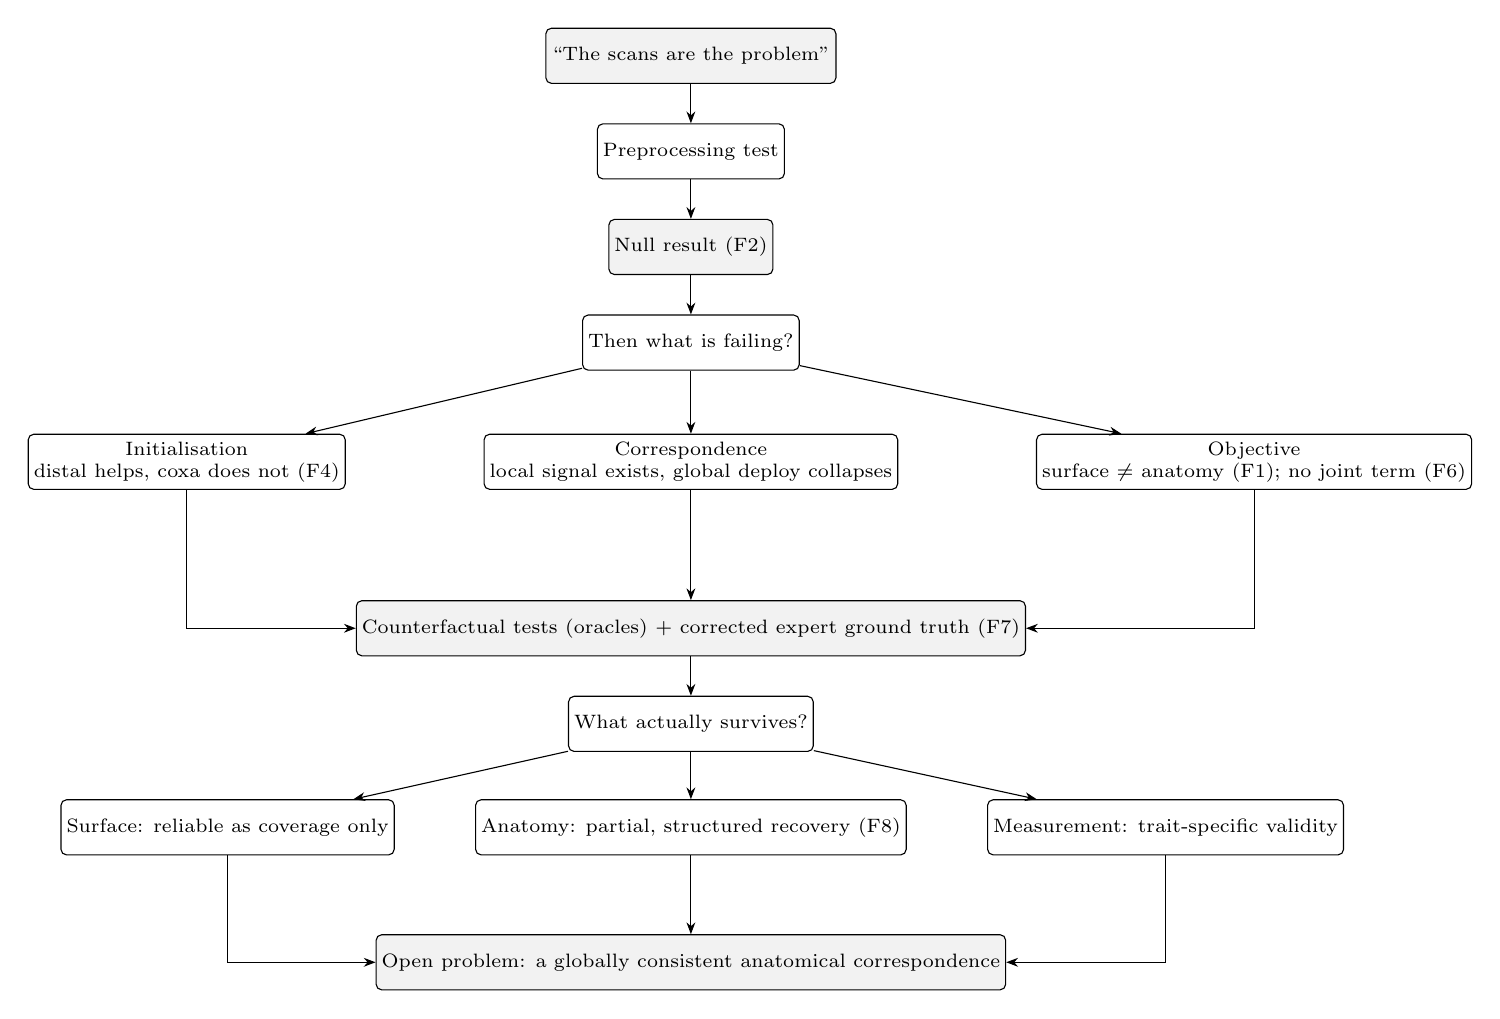
\begin{tikzpicture}[node distance=5mm and 5mm, every node/.style={font=\scriptsize},
 n/.style={draw,rounded corners=2pt,minimum height=7mm,align=center,fill=white,inner sep=2pt},
 arr/.style={-{Stealth[length=1.5mm]}}]
\node[n,fill=gray!10] (h0) {``The scans are the problem''};
\node[n,below=of h0] (pp) {Preprocessing test};
\node[n,below=of pp,fill=gray!10] (null) {Null result (\F{F2})};
\node[n,below=of null] (q) {Then what is failing?};
\node[n,below left=8mm and 30mm of q] (init) {Initialisation\\distal helps, coxa does not (\F{F4})};
\node[n,below=8mm of q] (corr) {Correspondence\\local signal exists, global deploy collapses};
\node[n,below right=8mm and 30mm of q] (obj) {Objective\\surface $\neq$ anatomy (\F{F1}); no joint term (\F{F6})};
\node[n,below=14mm of corr,fill=gray!10] (ct) {Counterfactual tests (oracles) + corrected expert ground truth (\F{F7})};
\node[n,below=of ct] (surv) {What actually survives?};
\node[n,below left=6mm and 22mm of surv] (s1) {Surface: reliable as coverage only};
\node[n,below=6mm of surv] (s2) {Anatomy: partial, structured recovery (\F{F8})};
\node[n,below right=6mm and 22mm of surv] (s3) {Measurement: trait-specific validity};
\node[n,below=10mm of s2,fill=gray!10] (open) {Open problem: a globally consistent anatomical correspondence};
\draw[arr](h0)--(pp); \draw[arr](pp)--(null); \draw[arr](null)--(q);
\draw[arr](q)--(init); \draw[arr](q)--(corr); \draw[arr](q)--(obj);
\draw[arr](init)|-(ct); \draw[arr](corr)--(ct); \draw[arr](obj)|-(ct);
\draw[arr](ct)--(surv); \draw[arr](surv)--(s1); \draw[arr](surv)--(s2); \draw[arr](surv)--(s3);
\draw[arr](s1)|-(open); \draw[arr](s2)--(open); \draw[arr](s3)|-(open);
\end{tikzpicture}
\caption{The investigation at a glance: from the initial mesh-quality
hypothesis, through its rejection, to a three-way diagnosis and what each
level of validity turned out to support.}
\label{fig:glance}
\end{figure}

\section{The redirection of the project}
\label{sec:turn}

The first weeks tested the hypothesis implicit in the brief (RQ1): a rebuilt
preprocessing pipeline was compared against the existing one with
registration held fixed. The two tied (\F{F2}, \S\ref{sec:prep-null}).
That null result located the problem elsewhere and redirected the internship
toward a question the pipeline had no instrument to answer: whether the
optimiser finds the \emph{right} correspondence, not merely a close surface.
Building that instrument from synthetic ground truth
(\S\ref{sec:synthetic-instrument}), and later an independent expert
benchmark (\S\ref{sec:skeleton-underdetermined}) after correcting a
coordinate-frame error in an early annotation set (\F{F7}), is the thread the
rest of the report follows.

\section{Established results}
\label{sec:ledger}

Results that recur are registered once here and cited by identifier
(\F{F1}, \F{F2}, and so on); evidence is in the chapter each points to. Table~\ref{tab:evidence}
(Chapter~\ref{ch:conclusion}) gives the evidence status of every headline
claim in the report.

\printfindingledger

\section{Contributions}

Existing SMILify provided the parametric representation and a baseline
optimisation-based fitting pipeline. This internship's contribution is the
diagnostic and validation machinery built around it, and what that machinery
established.

\textbf{Scientific contribution.} A diagnostic framework, evidenced
experimentally rather than asserted, showing that surface fit, anatomical
correspondence, parameter recovery and measurement validity are four
distinct properties that do not track one another: surface proximity does
not imply anatomical correspondence (\F{F1}); regional identity and
within-region localisation are distinct problems (\F{F3}); initialisation
sensitivity is anatomically heterogeneous (\F{F4}); the objective has no
explicit joint observation term and expert supervision does not propagate
spatially (\F{F6}); error is structured by joint and specimen rather than by
seed (\F{F8}); local learned correspondence does not imply dense global
correspondence (Chapter~\ref{ch:structure}); and accurate population-level
measurements can coexist with unreliable individual-level correspondence
(\S\ref{sec:scale-dependence}).

\textbf{Algorithmic contributions.} Chain-aware anatomical assignment; an
SDF-based anatomical field; a PointNet-style pose initialiser; localised
graduated non-convexity; a distal-protected sampling scheme; and learned
within-part correspondence descriptors, each evaluated against a
pre-registered criterion (Table~\ref{tab:evidence}), not assumed successful.

\textbf{Evaluation contributions.} A synthetic round-trip correspondence
benchmark; an adversarial metric test; a three-level evaluation protocol;
counterfactual (oracle) interventions for causal bottleneck localisation; a
corrected, frozen expert Joint Alignment Benchmark (11 specimens, 396 fits);
variance decomposition; and leave-one-region-out supervision.

\textbf{Systems and infrastructure contributions.} A configurable
preprocessing pipeline with Alpha Wrap and ManifoldPlus handling and
mesh-quality classification; integration of joint-limit priors into the 3D
registration path; a corrected staged fitting schedule; and reproducible
large-scale ablation studies across two HPC systems (JURECA, RWTH H100) with
fixed seeds, preserved checkpoints, configuration-driven experiments and
hash-frozen evaluation artifacts (\S\ref{sec:infrastructure}).

\textbf{What is open.} Within-part localisation on thin articulated
structures; the anterior deformation defect that the scale barrier did not
resolve; supplying joint information without expert annotation; and dense,
globally consistent learned correspondence. Claims not reproducible in the
final environment are marked provisional or excluded (Table~\ref{tab:evidence}).

\section{Structure of this report}

Chapter~\ref{ch:host} gives the host context and Chapter~\ref{ch:related}
positions the work against existing literature on parametric models,
point-cloud registration, shape correspondence, and defective mesh repair.
Chapter~\ref{ch:pipeline} defines the model, objective and pipeline
mathematically, and Chapter~\ref{ch:method} sets out the experimental
methodology. Chapter~\ref{ch:structure} reports the algorithmic
investigations and Chapter~\ref{ch:diagnostics} the mechanistic diagnosis of
the registration bottleneck. Chapter~\ref{ch:interventions} evaluates
candidate interventions against that diagnosis, Chapter~\ref{ch:validation}
is the move from registration to measurement, and Chapter~\ref{ch:conclusion}
the discussion, limitations and future work.

\chapter{Host organisation and research context}
\label{ch:host}

\section{Forschungszentrum Jülich and IAS-7}

The internship was carried out at Forschungszentrum Jülich, a member of the
Helmholtz Association, at IAS-7 (Civil Safety Research), part of the
Institute for Advanced Simulation and directed by Prof.\ Dr.\ Armin Seyfried.
IAS-7 works on pedestrian and fire dynamics through combined experimental and
simulation approaches. The link between an insect registration pipeline and
an institute concerned with crowd safety runs through method, not subject
matter: IAS-7's long-running tool \term{PeTrack} recovers pedestrian
trajectories from video automatically, because manual extraction cannot keep
pace with the institute's experimental series, but a trajectory is only a
point per person per frame. \term{smilify} is designed to give the same kind
of automated recovery a richer target: full three-dimensional pose and
shape, species-agnostic, from monocular or multi-view RGB video, and ants
serve as a demanding test case for it: thinner structures, more limbs,
greater articulation, and worse input data than a human subject in a
laboratory corridor. A registration method proven on a six-legged,
few-millimetre specimen from imperfect photogrammetry is tested well beyond
the conditions of its eventual deployment.

Shared allocation on the Jülich Supercomputing Centre's own machines could
not absorb the internship's full compute demand; the more resource-intensive
experiments in this report were instead run on external HPC infrastructure
(\S\ref{sec:infrastructure}), so the computational scale of the work was not
a direct consequence of being hosted at Jülich.

\section{Research context: parametric models beyond human subjects}

This internship extends parametric three-dimensional shape models to species
outside the small set computer vision has historically addressed.
\term{SMPL}~\cite{smpl} assumes a cooperative subject, a large scan corpus,
and a fixed body topology; \term{SMAL}~\cite{smal} relaxed the first two
assumptions for quadrupeds by learning a shape space from toy figurines.
\term{smilify} continues this progression to insects, where the body plan
itself differs and the structures of interest are thin, numerous, and
highly articulated (Chapter~\ref{ch:pipeline} traces this lineage in full).
Upstream sits \term{scAnt}~\cite{scant}, an open-source macro photogrammetry
scanner by the same author, which makes high-resolution 3D capture of small
specimens accessible without dedicated scanning infrastructure: an
affordable scanner producing abundant imperfect data, and a robust
registration pipeline converting it into comparable measurements; neither
has much independent value without the other, and the failure mode
identified in Chapter~\ref{ch:introduction} sits exactly at their junction.

\section{Supervision and working arrangement}

The internship was supervised by Dr.\ Fabian Plum, postdoctoral researcher
at IAS-7 and author of \term{scAnt}~\cite{scant}, \term{replicAnt}~\cite{replicant},
\term{OmniTrax}~\cite{omnitrax}, and \term{smilify}, and ran on site from 1
July to 25 September 2026. Two aspects of that arrangement shaped the work.
First, the technical data sheet's assignments were an initial hypothesis
about where effort would be valuable, not a fixed specification: when the
controlled comparison in \S\ref{sec:turn} showed mesh input quality was not
the limiting factor, redirecting the remaining work toward initialisation
and correspondence was the correct response to the evidence. Second,
development took place on a live, shared repository under standard
pull-request review, with the supervisor running related experiments on
adjacent branches; several results reported later in this document were
revised following that review, and the pre-registration discipline used
throughout the report follows directly from it. Beyond ants, the same
pipeline has since been used to build parametric models of other species,
context worth noting since the problems investigated here are not specific
to Formicidae.

\section{Academic framing}

This internship forms part of the second year of the engineering cycle at
Universit\'e Mohammed VI Polytechnique, and this report is the corresponding
academic deliverable. It documents both the technical contributions produced
and the evidence behind the decisions that shaped the work's direction,
inseparable here, since the most consequential decisions taken during the
internship concerned which lines of investigation to discontinue, and those
decisions are only defensible alongside the evidence that motivated them.

\chapter{Related work and research context}
\label{ch:related}

This chapter positions the investigation within four lines of existing work,
not as a survey but to establish which parts of the problem are recognised
open questions elsewhere and which parts this report investigates directly.

\textbf{Parametric articulated models.} \term{SMPL}~\cite{smpl} learns a
human shape and pose space from a large registered scan corpus under a fixed
body topology. \term{SMAL}~\cite{smal}, from the same \emph{3D Menagerie}
line of work, relaxes the cooperative-subject and topology assumptions for
quadrupeds by learning a shape space from toy figurines and fitting it to
images and video~\cite{smalify}. \term{smilify} continues this progression
to insects, where the body plan itself differs and every structure of
interest is thin and articulated (Chapter~\ref{ch:pipeline}).

\textbf{Point-cloud and mesh registration.} Classical iterative closest
point and its variants align point sets by alternating nearest-neighbour
correspondence and rigid transformation estimation, and are known to
converge to spurious local optima under poor initialisation or partial
overlap. Learning-based registration addresses this directly: \term{Deep
Closest Point}~\cite{dcp} learns point embeddings for closest-point
matching end-to-end; \term{PREDATOR}~\cite{predator} predicts an overlap
region between two point clouds before matching, specifically to handle
low-overlap pairs; and \term{GeoTransformer}~\cite{geotransformer} combines
geometric attention with coarse-to-fine matching for dense correspondence.
These methods establish that initialisation, overlap, and correspondence
are recognised as separable, fundamental difficulties in point-cloud
registration generally. This report studies a harder, model-based variant:
registration constrained to the image of a parametric articulated model
rather than a free rigid or non-rigid point-set alignment, where the
nearest-surface matching implicit in a Chamfer-style objective is the local
matching mechanism and the open question is what information that mechanism
lacks (\S\ref{sec:registration}).

\textbf{Shape correspondence.} Beyond point-to-point matching,
\term{functional maps}~\cite{fmaps} represent a correspondence between two
shapes as a compact linear map between functions defined on them, and a
substantial subsequent literature extends this to partial and non-isometric
settings; \term{optimal transport}~\cite{ot} provides a complementary
globally-consistent matching formulation under an explicit transport cost,
with partial-transport variants suited to incomplete observations. These
are the two directions this report's outlook (\S\ref{sec:learned-correspondence},
Chapter~\ref{ch:conclusion}) points to for closing the local-to-global gap
exposed by the learned-descriptor experiments.

\textbf{Defective mesh repair.} \term{Alpha Wrap}~\cite{alphawrap}
constructs a watertight offset surface enclosing arbitrarily defective
input, with an explicit offset parameter trading fidelity against
robustness; \term{ManifoldPlus}~\cite{manifoldplus} instead repairs a given
triangle soup directly into a watertight manifold. Both target exactly the
defect classes (holes, self-intersections, non-manifold geometry)
present in the scan corpus this report works with (\S\ref{sec:preprocessing}).

None of these methods is claimed to solve the problem studied here; they are
cited to establish that each mechanism this report investigates
(initialisation, correspondence, overlap-like partiality, and defective
input) is an independently recognised difficulty in 3D registration, and
that this report's contribution is to characterise how these difficulties
interact specifically for an articulated, model-based, biological fitting
problem.

\chapter{The registration pipeline}
\label{ch:pipeline}

% Each section of this chapter lives in its own file under
% chapters/03_pipeline/ so it can be edited independently.
\section{From SMPL to a body-plan-agnostic model}

\term{SMILify} keeps the recipe that made \term{SMPL}~\cite{smpl} and
\term{SMAL}~\cite{smal} useful (a fixed-topology template mesh, deformed by
a low-dimensional shape vector $\bm\beta$ and a per-joint pose $\bm\theta$
under linear blend skinning) and removes the assumption both predecessors
still made: that the skeleton's topology is known and shared in advance
(24 human joints, or a common quadruped rig). SMIL instead accepts an
arbitrary rigged mesh as its template, so the same fitting machinery serves a
six-legged, antenna- and mandible-bearing ant as readily as a mammal.

\begin{figure}[!htb]
\centering
\includegraphics[width=0.62\linewidth]{figures/fig_model_lineage.jpg}
\caption{The lineage of body-plan-agnostic parametric models: a fixed human
topology (SMPL), a shared quadruped rig learned from toy figurines (SMAL),
and \term{SMILify}, which fits an arbitrary rigged template (here an
ant) to scan-derived meshes of any body plan.}
\label{fig:lineage}
\end{figure}

Every fitted specimen is expressed in the same model coordinate system
(Figure~\ref{fig:coord}): the same vertex index always refers to the same
named anatomical locus, so that once a corpus is registered, quantities such
as head width or leg segment length become directly comparable across
specimens without any further alignment step. This is the property the whole
pipeline exists to protect; \S\ref{sec:correspondence-def} makes precise what
can go wrong with it.

\begin{figure}[!htb]
\centering
\includegraphics[width=0.62\linewidth]{figures/fig_parameter_space.jpg}
\caption{One shared parameter space, many specimens: the low-dimensional
shape vector $\bm\beta$ learned by the model places every registered
specimen at a point in a common space, in which distance is anatomically
meaningful.}
\label{fig:coord}
\end{figure}

\section{The SMIL representation}
\label{sec:representation}

The model has a fixed-topology template of $10{,}235$ vertices, a kinematic
tree of $55$ joints with a joint regressor, per-vertex skinning weights, a
$25$-dimensional shape basis, a bilateral symmetry map and authored joint
rotation limits. Fixed topology is what makes correspondence possible at all:
vertex $i$ denotes the same anatomical locus in every fit, so a registered
corpus lives in one coordinate system.

A shaped vertex is $\bar{\mathbf v}_i(\bm\beta)=\mathbf v^{0}_i+\sum_k\beta_k\mathbf s_{ik}$
and is posed by \term{linear blend skinning}:
\begin{equation}
\mathbf v_i(\bm\beta,\bm\theta)=\sum_{j=1}^{55} w_{ij}\,G_j(\bm\theta)\,\bar{\mathbf v}_i(\bm\beta),
\qquad G_j(\bm\theta)=\prod_{k\in\mathrm{anc}(j)}\big[R(\theta_k)\,|\,\mathbf t_k\big],
\label{eq:lbs}
\end{equation}
where $w_{ij}$ are skinning weights and $G_j$ composes the transforms of all
ancestors of joint $j$ along the kinematic chain. Two consequences drive
later results. A rotation error at a proximal joint changes $G_j$ for every
descendant, so it displaces every downstream vertex (the proximal/distal
sensitivity of \S\ref{sec:articulation}). And the surface depends on joint
\emph{positions} only through $G_j$, which is why a surface can look right
while the skeleton inside it is wrong (\F{F6}).

\begin{figure}[!htb]
\centering
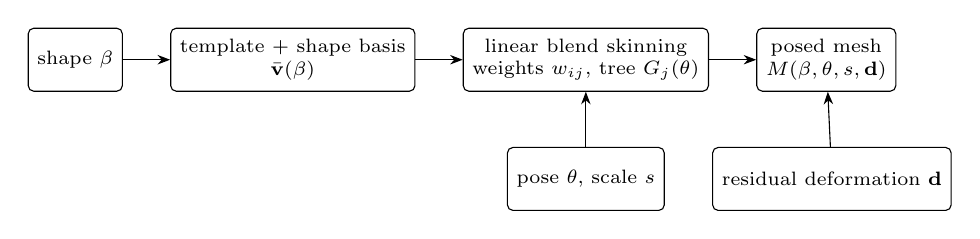
\begin{tikzpicture}[node distance=7mm and 6mm, every node/.style={font=\scriptsize},
 box/.style={draw,rounded corners=2pt,minimum height=8mm,align=center,fill=white},
 arr/.style={-{Stealth[length=1.6mm]}}]
\node[box] (b) {shape $\bm\beta$};
\node[box,right=of b] (t) {template $+$ shape basis\\$\bar{\mathbf v}(\bm\beta)$};
\node[box,right=of t] (l) {linear blend skinning\\weights $w_{ij}$, tree $G_j(\bm\theta)$};
\node[box,right=of l] (m) {posed mesh\\$M(\bm\beta,\bm\theta,s,\mathbf d)$};
\node[box,below=of l] (p) {pose $\bm\theta$, scale $s$};
\node[box,right=of p] (d) {residual deformation $\mathbf d$};
\draw[arr] (b)--(t); \draw[arr] (t)--(l); \draw[arr] (l)--(m);
\draw[arr] (p)--(l); \draw[arr] (d)--(m);
\end{tikzpicture}
\caption{The SMIL forward model. Registration inverts it from surface samples
alone.}
\label{fig:forward-model}
\end{figure}

\section{Pipeline overview}
\label{sec:pipeline-overview}

\begin{figure}[!htb]
\centering
\includegraphics[width=0.78\linewidth]{figures/fig_pipeline_full.jpg}
\caption{The registration pipeline, from diverse raw scan data to a fitted
parametric model with explicit vertex-wise correspondence. The pipeline
stages are described in \S\ref{sec:preprocessing}--\S\ref{sec:registration};
the correspondence stage did not exist before this internship and is the
subject of Chapters~\ref{ch:diagnostics}--\ref{ch:validation}.}
\label{fig:pipeline}
\end{figure}

The delivered pipeline (Figure~\ref{fig:pipeline}) has four stages: preprocessing,
initialisation, registration, and, newly introduced during this
internship, an explicit correspondence-audit stage that reports, for a
fitted specimen, how confidently each vertex's identity can be trusted rather
than only how close the surfaces are. The following sections take each stage
in turn.

\section{Preprocessing}
\label{sec:preprocessing}

Real Antscan meshes (photogrammetry via \term{scAnt}~\cite{scant}, or
micro-CT) arrive with a wide range of defects: holes, disconnected
fragments, non-manifold edges and vertices, small debris, self-intersecting
and fused geometry, thin appendages that vanish under naïve simplification,
and highly variable pose and orientation. Two complementary repair
strategies were evaluated rather than assumed:

\begin{itemize}
\item \textbf{Alpha Wrap}~\cite{alphawrap} constructs an entirely new, watertight envelope
around the input geometry, regardless of how damaged the input is. Its
single scale parameter trades off two failure directions: too coarse an
envelope and thin anatomical structures (legs, antennae) disappear
into it; too fine, and the noise and defects the envelope was meant to
remove survive into the output.
\item \textbf{ManifoldPlus}~\cite{manifoldplus} instead repairs and regularises the input
surface directly, and was used as a fallback specifically for cases Alpha
Wrap's envelope construction did not adequately resolve.
\item \textbf{Conservative cleanup and reduction.} Before and after repair,
duplicate vertices, degenerate faces and loose vertices are removed and
normals recomputed, and topology-preserving quadric-error-metric (QEM)
reduction~\cite{qem} lowers face count without collapsing thin appendages.
\end{itemize}

\begin{investigation}{I12}{Does the rebuilt preprocessing pipeline actually
produce more reliably watertight, better-conditioned meshes?}
\invQuestion{Benchmarked against the existing pipeline on the same corpus,
does the Alpha-Wrap-plus-ManifoldPlus pipeline improve mesh topology?}
\invMethod{Watertightness and connected-component count across 44 processed
specimens, compared against the existing preprocessing pipeline; Alpha
Wrap's scale parameter swept toward progressively finer offsets.}
\invResult{$44$ of $44$ processed meshes were watertight, and $29$ of $44$
were reduced to a single connected component, both a substantial
improvement in topology over the existing pipeline. Some configurations at
the finest offsets encountered memory limitations at $32$\,GB.}
\invVerdict{ADOPT}{Retained as the production preprocessing pipeline.
Whether this translated into more accurate downstream registration is a
separate question, answered in \S\ref{sec:prep-null}: it did not, to a
measurable degree (\F{F2}): watertightness is a precondition for reliable
fitting, not, on its own, a source of anatomical accuracy.}
\end{investigation}

This preprocessing stage is wrapped in a production data-preparation module,
\allowbreak\texttt{prepare\_antscan\_\allowbreak data\_for\_mesh\_\allowbreak
fitting.py}, which converts raw
Antscan exports into a fitting-ready corpus: consistent scale and
orientation, organised clean/processed variants, and batch-ready input for
the registration stage proper. The registration stage itself, run through
\texttt{fitter\_3d/\allowbreak optimise.py}, preserves every intermediate optimisation
stage (\texttt{Stage\_0\_init}, \texttt{Stage\_1\_default},
\texttt{Stage\_2\_deform\_coarse}, \texttt{Stage\_3\_deform\_fine}) along
with per-specimen parameter files, reconstructed meshes, and loss curves,
so that any registration result in this report can be re-inspected or
re-run rather than taken on trust. This reproducibility infrastructure is
what made the controlled comparisons throughout Chapters~\ref{ch:structure}
and~\ref{ch:diagnostics} possible in the first place: a controlled variant
is only informative if the configuration that produced it is preserved
exactly.

\section{Initialisation}
\label{sec:init-stage}

A \term{PointNet}-style~\cite{pointnet} point-cloud encoder predicts an
initial shape, pose and global transform directly from the target mesh,
avoiding a fixed canonical starting pose that real specimens rarely match.
\S\ref{sec:articulation} quantifies how much of registration failure this
stage is, and is not, responsible for.

\section{Registration objective}
\label{sec:registration}

Registration (Eq.~\ref{eq:registration}) is solved by differentiable
gradient-based optimisation with PyTorch3D~\cite{pytorch3d}, minimising
$\mathcal{L}=\sum_t\lambda_t\mathcal{L}_t$ over the terms below. The table
states what each term \emph{observes}, which is the information the
optimiser actually has:
\begin{center}
\small
\begin{tabular}{@{}p{0.20\linewidth}p{0.70\linewidth}@{}}
\toprule
\textbf{Term} & \textbf{What it observes} \\
\midrule
Chamfer & Distance from each sampled model point to its nearest target point
  and back; a function of two surfaces, blind to which vertex is which \\
Normal & Agreement of surface normals at matched points \\
Edge / Laplacian / offset & Local mesh regularity and size of residual
  deformation $\mathbf d$; target-independent, ARAP-style~\cite{arap} \\
Symmetry / midline & Bilateral consistency of the model \\
Rotation limits & Joint \emph{angles} against authored ranges, not joint
  positions \\
\bottomrule
\end{tabular}
\end{center}
No term takes a joint location or a vertex identity as an observation.
The surface term is evaluated on $N$ sampled points,
$\mathcal{L}_{\mathrm{ch}}\approx\frac1N\sum_i d(p_i,T)^2$, so the sampling
distribution is itself an implicit weighting over anatomy
(\S\ref{sec:sampling}). Optimisation is staged and hierarchical: global
pose and scale first, then coarse, then fine vertex deformation, rather
than a single flat descent; \S\ref{sec:staged} reports a defect found in this
schedule.

\section{Correspondence}
\label{sec:correspondence-def}

Every one of the eight terms in \S\ref{sec:registration} is a function of
surface geometry, not of vertex identity: $\mathcal{L}_{\mathrm{chamfer}}$ is
minimised by the \emph{nearest} target point to each template vertex, not by
the \emph{anatomically corresponding} one. Two meshes can therefore agree
almost perfectly as surfaces while disagreeing almost completely about which
point is which: the central observation of this report, introduced in
Chapter~\ref{ch:introduction} and diagnosed mechanistically in
Chapter~\ref{ch:diagnostics}. Because no correspondence measurement existed
in the pipeline before this internship, one had to be built from synthetic
ground truth before that diagnosis was even possible; that instrument is
described first, in \S\ref{sec:synthetic-instrument}, because every later
result in this report depends on it.

\section{Technical stack}

\begin{center}
\begin{tabular}{@{}p{0.30\linewidth}p{0.62\linewidth}@{}}
\toprule
\textbf{Component} & \textbf{Role} \\
\midrule
PyTorch / PyTorch3D~\cite{pytorch3d} & Differentiable mesh geometry,
  rendering, and autograd-based optimisation of $(\bm\beta,\bm\theta,s,\mathbf d)$ \\
PointNet~\cite{pointnet} & Point-cloud encoder for learned pose/shape
  initialisation, replacing a fixed canonical start \\
Shape Diameter Function~\cite{sdf} & Local-thickness descriptor evaluated as
  a candidate part-aware segmentation and correspondence signal \\
As-rigid-as-possible energy~\cite{arap} & Reference formulation for the
  edge/Laplacian deformation-cost terms used to bound free vertex deformation \\
Synthetic round-trip harness & Purpose-built during the internship: samples
  the model's own distribution, exports an anonymous mesh with known
  per-vertex identity, and re-fits it, giving exact correspondence ground
  truth with no manual annotation cost \\
\bottomrule
\end{tabular}
\end{center}

\section{What was built}

\begin{figure}[!htb]
\centering
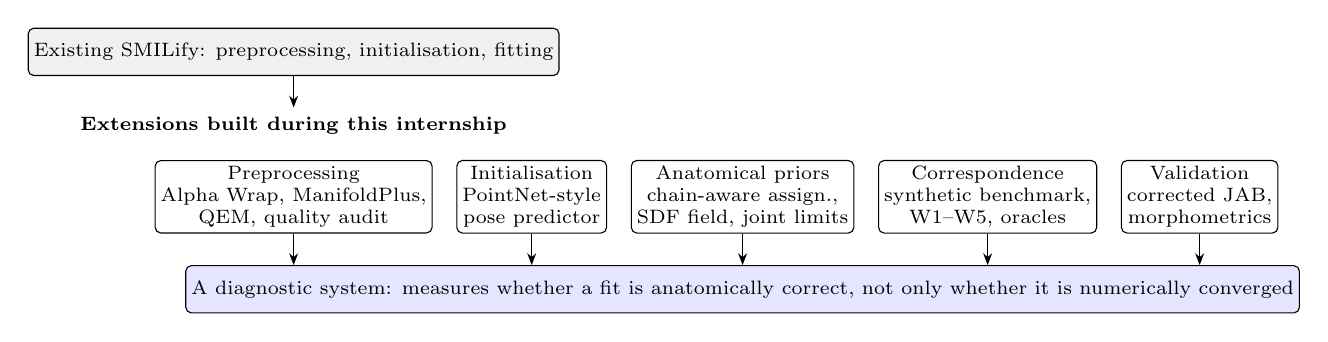
\begin{tikzpicture}[node distance=4mm and 4mm, every node/.style={font=\scriptsize},
 n/.style={draw,rounded corners=2pt,minimum height=6mm,align=center,fill=white,inner sep=2pt},
 hdr/.style={font=\scriptsize\bfseries}]
\node[n,fill=gray!12] (base) {Existing SMILify: preprocessing, initialisation, fitting};
\node[below=4mm of base,hdr] (ext) {Extensions built during this internship};
\node[n,below=2mm of ext] (p1) {Preprocessing\\Alpha Wrap, ManifoldPlus,\\QEM, quality audit};
\node[n,right=3mm of p1] (p2) {Initialisation\\PointNet-style\\pose predictor};
\node[n,right=3mm of p2] (p3) {Anatomical priors\\chain-aware assign.,\\SDF field, joint limits};
\node[n,right=3mm of p3] (p4) {Correspondence\\synthetic benchmark,\\W1--W5, oracles};
\node[n,right=3mm of p4] (p5) {Validation\\corrected JAB,\\morphometrics};
\node[n,below=4mm of p3,fill=blue!10,minimum width=8.6cm] (diag) {A diagnostic system: measures whether a fit is anatomically
correct, not only whether it is numerically converged};
\draw[-{Stealth[length=1.5mm]}] (base)--(ext);
\foreach \p in {p1,p2,p3,p4,p5}{\draw[-{Stealth[length=1.5mm]}] (\p)--(\p|-diag.north);}
\end{tikzpicture}
\caption{Existing SMILify supplied the parametric representation and a
baseline optimisation-based fitting pipeline. This internship added the
diagnostic and validation machinery around it: a framework for
distinguishing numerical convergence, surface agreement, anatomical
correspondence, and measurement validity, not a system that certifies
anatomical correctness unconditionally. Every box is implemented and
evaluated in this report; none of it is a re-run of the existing pipeline.}
\label{fig:what-built}
\end{figure}

\section{What this chapter does not yet answer}

The pipeline above is a complete, executable registration workflow, and every stage in it
existed, in some form, before this internship. What was missing was a reliable way to tell, for a given fitted specimen,
whether a numerically successful optimisation corresponded to an
anatomically correct recovery, or merely a plausible one. Chapter~\ref{ch:diagnostics}
builds that instrument and uses it to localise where, mechanistically, the
pipeline above produces anatomically wrong fits despite a low value of
$\mathcal{L}$.


\chapter{Experimental methodology}
\label{ch:method}

Every result in this report rests on one of three kinds of ground truth, and
the methodology is organised around knowing which.

\section{Synthetic ground truth and the round-trip benchmark}
\label{sec:synthetic-method}

Real scans have no known vertex identities, so correspondence cannot be
measured on them directly. The model can, however, generate its own targets:
sample latent variables, pose the template, export an anonymous mesh, refit
it, and compare against the known truth. The corpus used holds $5000$
specifications drawn with a fixed seed, pose scale $0.50$ and shape scale
$2.0$, with fixed train/test splits; this allows the perturbation, sampling,
initialisation and correspondence variables to be manipulated one at a time.

\begin{algbox}{1: Synthetic round-trip correspondence benchmark}
\begin{enumerate}[nosep,leftmargin=1.4em]
\item Sample $(\bm\beta,\bm\theta)$ from the model's learned distributions (fixed seed).
\item Generate the posed mesh $M$; keep the true identity of every vertex.
\item Optionally corrupt $M$ (noise, holes, dropped points) and strip identities.
\item Run the production fitter on the anonymous mesh, optionally with a
counterfactual input (ground-truth initialisation, regional-identity oracle).
\item For each vertex $i$, compare fitted vertex $i$ with true vertex $i$;
report correspondence, parameter and surface errors per anatomical part.
\end{enumerate}
\end{algbox}

The limitation is intrinsic: the target comes from the model, so the
benchmark bounds error from below on real scans (\S\ref{sec:limitations}).

\section{Metrics and reference standards}

Three kinds of reference are used, at increasing authority. \textbf{Surface
metrics}: Chamfer distance, F-score, Hausdorff distance and per-part
variants. \textbf{Integrity metrics}: edge-length distortion, Laplacian and
as-rigid-as-possible deviation, normal consistency; these need no target and
so cannot be gamed by fitting it. \textbf{Anatomical references}: exact
vertex identity on synthetic data, and manual 3D joint annotations by an
expert on real specimens, for which skeleton error is reported as a
percentage of \term{Weber's length} (the anatomical length of the mesosoma,
used as a size-invariant unit).

Because ground truth is software infrastructure as much as data, the
expert annotations were placed under a validated reference-frame protocol
(\S\ref{sec:skeleton-underdetermined}): the mesh coordinate convention was
checked, annotations were re-registered through each mesh to a residual below
$7\times10^{-8}$, and the benchmark was frozen and hash-verified (SHA-256).

\section{Statistical testing and reproducibility}

Paired comparisons across specimens use bootstrap confidence intervals and
sign or Friedman tests where several configurations are ranked; variance is
attributed to joint, specimen and optimiser seed on the log scale. Leave-one-region-out
evaluation withholds supervision for one anatomical region at a time to test
whether supervision propagates. Every reported run uses recorded seeds,
preserved configuration files, checkpoints and intermediate fitting stages
(\texttt{Stage\_0}--\texttt{Stage\_3}), so a controlled comparison can be
re-run rather than trusted. Results whose run artifacts could not be
reproduced in the final environment are labelled as such in
Table~\ref{tab:evidence}.


\chapter{Anatomical structure, initialisation, and learned correspondence}
\label{ch:structure}

Chapter~\ref{ch:pipeline} described the pipeline as four sequential stages.
This chapter reports the technical work behind the first three, organised
around a single question asked with escalating power: \emph{where can the
fitter be given more of the information the surface objective lacks?} First
as fixed anatomical priors; then as a better starting point; then inside the
optimiser itself; then as a descriptor learned from data; and finally as a
counterfactual test of how much each source of information is actually
worth. Every result below was tested against a controlled benchmark before
being adopted or rejected; several are negative results, reported because a
negative result under a controlled comparison rules out a hypothesis as
usefully as a positive one confirms it.

\subsection*{Anatomical priors}
\section{Chain-aware anatomical assignment}
\label{sec:chain-aware}

Several downstream analyses in this report (the per-part correspondence
audit, the multi-level evaluation suite in \S\ref{sec:eval-suite})
depend on a prior step: deciding which anatomical structure a given surface
point belongs to. A naïve nearest-segment rule, which assigns each point to
whichever skeleton bone is geometrically closest, fails systematically on an
articulated body plan: a point on a middle leg can sit closer in raw
distance to the wrong leg, or to the body, than to its own leg, because the
rule treats every bone independently rather than as part of a connected
kinematic chain. A \textbf{chain-aware} rule, which resolves ambiguous
points by their position along the connected chain rather than by raw
distance, was tested against it on the same labelled template and adopted:
macro-averaged F1 improves from $0.656$ to $0.831$, concentrated exactly
where the naïve rule was weakest (middle-leg recall $0.349\to0.768$,
body/core recall $0.366\to0.663$). The lesson generalises beyond this one
rule: an articulated body plan is not a set of independent parts, and
geometric rules that treat it as one will fail systematically at the joints
between parts.

\begin{algbox}{2: Chain-aware anatomical assignment}
\begin{enumerate}[nosep,leftmargin=1.4em]
\item For each surface point $p$, compute distance to every bone segment.
\item Group segments into kinematic chains (each leg, antenna, mandible, body axis).
\item Assign $p$ to the chain whose segments are collectively closest, using
the chain's connected extent rather than the single nearest segment.
\item Within that chain, assign to the nearest segment.
\end{enumerate}
\end{algbox}

\section{The Shape Diameter Function as an anatomical prior}

A separate line of investigation asked whether a local-thickness descriptor could
support anatomical assignment more robustly than surface-based rules. The
\term{shape diameter function}~\cite{sdf} assigns every surface point a
value related to the local thickness of the solid behind it: the value $\mathrm{SDF}(x)$ is obtained by casting rays into the solid
behind a surface point and taking a robust average of chord lengths, so thin
structures (legs, antennae) take small values, the bulky body takes large
ones, independently of pose; and, unlike the model's own vertex
correspondence, it is computable directly on a raw, unregistered scan. It
proved reliable for one purpose and unreliable for another. It reproduces
well across real scans (correlation $r\approx0.77$--$0.94$, $87$--$95\%$
agreement, under $1.3$\,s per specimen) and separates body from appendage on
the template with high accuracy (AUC $\approx0.973$, balanced accuracy
$\approx95.1\%$). But thresholding the field to separate \emph{individual}
appendage instances (one leg from its neighbour, left mandible from right)
fails on real scans: only $2$ of $12$ specimens had all four
expert-identified landmarks fall into distinct connected components, with
the two mandibles merged into one component in $9$ of $12$. The descriptor
is retained as a reliable, cheap semantic signal for \emph{which class of
structure} a region belongs to; it is not a mechanism for separating
individual instances of a repeated structure, because connected components cannot separate two
structures that are physically fused in the scan (laterality is not encoded in local
thickness). This is the instance-level correspondence problem this report's other sections address by different
means.

\section{Model configuration: joint limits and the shape prior}
\label{sec:model-configuration}

The production template used throughout this report is a joint-limited
SMIL model: $10{,}235$ vertices, $55$ joints, a $25$-dimensional shape space,
with an accompanying joint regressor, kinematic tree, skinning weights,
bilateral symmetry mapping, and, as the specific addition evaluated here,
authored per-joint rotation limits. Consuming these limits as a hard prior
during optimisation is the rotation-limit intervention already reported as
adopted in \S\ref{sec:eval-suite} and analysed mechanistically in \F{F1};
this section reports two related configuration choices tested alongside it.

\textbf{Joint limits and bilateral symmetry improve plausibility, not
correspondence.} Constraining joint rotation to anatomically authored ranges
measurably improves physical plausibility (fewer anatomically impossible
poses), and a companion bilateral (midline) symmetry constraint measurably
improves left/right consistency. Neither, on its own, resolves the
underlying correspondence problem characterised in \F{F1}, \F{F3}, and
\F{F6}: a pose can be entirely plausible, and entirely symmetric, while
still assigning the wrong vertex to the wrong anatomical location. This is
the same distinction as \F{F1} applied to a different pair of constraints:
plausible articulation is not the same property as correct articulation.

\textbf{A shape prior was added, then removed.} A Gaussian penalty on the
shape parameters $\bm\beta$ was tested as a stabiliser, on the standard
assumption that penalising extreme shape values improves numerical
robustness. It was subsequently removed after being found to suppress
genuine, biologically meaningful shape variation, the same variation
Chapter~\ref{ch:validation} depends on to distinguish specimens from one
another at all. This is reported as a deliberate reversal rather than an
oversight: a regularisation term can improve an optimisation diagnostic
while actively damaging the property the model exists to preserve, and for
a morphology-measurement pipeline specifically, that trade-off is not worth
making.


\subsection*{A better starting point}
\section{A learned pose initialiser, and where it breaks}
\label{sec:pointnet-init}

\S\ref{sec:init-stage} introduced a \term{PointNet}-style~\cite{pointnet}
initialiser: a point-cloud encoder that reads the raw target points,
extracts a permutation-invariant feature per point, pools them into one
global descriptor, and regresses an initial pose and shape directly from
it, replacing a fixed canonical starting pose with a learned, input-aware
one. The motivation follows from \F{F4}: for the distal chain, initialisation determines
which target surface region becomes each vertex's first attractor, so a
better starting point should, in principle, reduce how often the optimiser
locks onto the wrong one.

\begin{figure}[!htb]
\centering
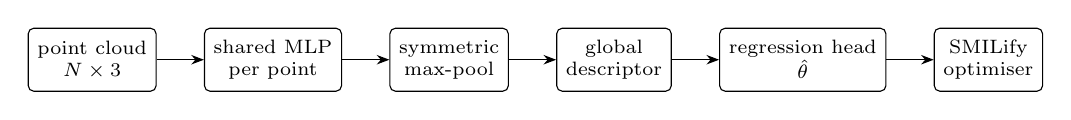
\begin{tikzpicture}[every node/.style={font=\scriptsize},
 box/.style={draw,rounded corners=2pt,minimum height=8mm,align=center,fill=white},
 arr/.style={-{Stealth[length=1.6mm]}}]
\node[box] (a) {point cloud\\$N\times3$};
\node[box,right=6mm of a] (b) {shared MLP\\per point};
\node[box,right=6mm of b] (c) {symmetric\\max-pool};
\node[box,right=6mm of c] (d) {global\\descriptor};
\node[box,right=6mm of d] (e) {regression head\\$\hat{\bm\theta}$};
\node[box,right=6mm of e] (f) {SMILify\\optimiser};
\foreach \x/\y in {a/b,b/c,c/d,d/e,e/f}{\draw[arr] (\x)--(\y);}
\end{tikzpicture}
\caption{Learned initialiser. Max-pooling makes the descriptor invariant to
point ordering, which a raw scan does not have.}
\label{fig:pointnet}
\end{figure}


\begin{investigation}{I11}{Does the learned initialiser improve registration,
and does a synthetic improvement transfer to real specimens?}
\invQuestion{Under controlled, exact synthetic ground truth, does the
learned initialiser outperform the existing default; and does that
advantage hold on real scans?}
\invMethod{Synthetic benchmark: learned vs.\ default initialisation, exact
ground truth known. Real-data benchmark: 50 real specimens, learned vs.\
zero (default) initialisation at three levels of synthetic pose
perturbation used during training ($\approx\!23^\circ$, then retrained at
$\approx\!13.8^\circ$ and $\approx\!8.85^\circ$).}
\invResult{On synthetic data the learned initialiser wins clearly: leg
accuracy improves from $0.857$ to $0.901$ and Chamfer distance from
$0.000264$ to $0.000226$. On the 50-specimen real benchmark at the
$23^\circ$ training regime, this reverses: learned initialisation
($0.000697$ mean Chamfer) is \emph{worse} than the zero-initialised default
($0.000637$), winning only 20 of 50 specimens. Retraining at smaller
perturbation magnitudes moves the comparison toward parity rather than
robust superiority.}
\invVerdict{REJECT}{The observed failure is consistent with a
synthetic-to-real distribution mismatch: performance did not transfer from
the tested synthetic training regime to real scans, and the
perturbation-magnitude sweep supports that interpretation. The experiments
do not establish whether the architecture itself would generalise under a
more representative training distribution, only that it did not under the
one tested. Not deployed in production as evaluated. The general lesson is
retained as a standing caution: a better initialiser can, in principle,
improve optimisation without addressing correspondence at all, and a
synthetic evaluation cannot certify real-world transfer by itself.}
\end{investigation}

A controlled follow-up sweep, holding total pose-error magnitude fixed and
varying only where along the kinematic chain it was placed, is what produced
the proximal/distal result reported as \F{F4} in \S\ref{sec:articulation}:
the same error placed proximally degrades leg accuracy far more (to $0.768$)
than the identical error placed distally ($0.939$), because a proximal
mistake propagates through every joint downstream of it.


\subsection*{A better-behaved optimiser}
\section{Sampling starvation and robust optimisation}
\label{sec:sampling}

\textbf{Sampling starvation.} The surface term is a Monte Carlo estimate,
$\mathcal{L}_{\mathrm{ch}}\approx\frac1N\sum_i d(p_i,T)^2$ with
$p_i\sim p(x)$. If $p$ is proportional to surface area, the expected loss
$\mathbb{E}_{x\sim p}[\mathrm{err}(x)]$ weights the body and head far more
than distal legs or antennae, so a tiny structure can be almost invisible to
the optimiser: a second route to the under-representation of \F{F5}, this
time in the sampling scheme rather than the mesh. Reserving a fixed quota of
the global budget for distal points improved distal legs but starved
antennae and head, which shared that budget; restricting the quota to within
the leg budget avoided the trade-off, yet did not clearly improve on simply
splitting distal sampling. The conclusion is narrow: starvation is a real
confound, but controlling it did not create anatomical correspondence.

\textbf{Robust optimisation.} A related question is how the objective
should respond to points that are simply wrong (occluded regions,
scanning artefacts, disconnected debris) rather than merely
under-sampled. \term{Graduated non-convexity} (GNC)~\cite{gnc} is a robust-optimisation
strategy that treats every point correspondence as suspect initially and
progressively hardens its confidence in inliers as optimisation proceeds,
rather than trusting every nearest-point match from the first iteration.
Applied globally across the whole body, it produced undesirable behaviour
specifically around the antennae; restricted to the leg point set alone
(\emph{leg-only, topology-free}), it improved robustness where applied,
under synthetic corruption benchmarks with 30\% and 60\% of points dropped:
accuracy rose from $0.602$ to $0.797$ (Drop30) and from $0.411$ to $0.607$
(Drop60). Localising the robust treatment to the anatomical subsystem where
corrupted points actually occur outperformed applying it uniformly; the
result is retained as a promising candidate for leg registration
specifically, not adopted as a general replacement for point-matching across
the whole body.


\subsection*{Correspondence learned from data}
\section{From geometric to learned correspondence}
\label{sec:learned-correspondence}

Every correspondence mechanism considered so far in this report is
geometric: a vertex is matched to whichever target point is nearest to it,
possibly after the chain-aware and shape-diameter refinements of the previous
sections. A separate line of work asked whether a \emph{learned}
descriptor, a small network trained to produce a feature vector per
point such that corresponding anatomical locations produce similar vectors
could do better, and pursued that question through four increasingly
demanding tests.

The first attempt, a handcrafted baseline rather than a learned one,
normalised each point's coordinates within its own anatomical part (by that
part's local length and radius) before matching, on the hypothesis that
canonicalising away each part's specific proportions would make
correspondence easier to learn. It performed \emph{worse} than raw
coordinates: normalising away a part's specific geometry destroys
information that, it turns out, itself carries correspondence signal. The
first genuinely learned descriptor, trained with an off-the-shelf objective,
then failed when deployed, for a mundane but instructive reason: a mismatch
between the density of points it was trained on and the density it was
evaluated and deployed on, not a failure of the learning approach itself.
This motivated a redesigned, within-part training objective, tested next.

Two tasks must be kept apart. \emph{Pairwise retrieval} matches each query
point to its nearest neighbour in descriptor space,
$q_i\mapsto\arg\min_j\|f(q_i)-f(t_j)\|$. \emph{Dense correspondence} needs a
whole assignment $\{q_i\}_{i=1}^N\mapsto\{t_{\pi(i)}\}_{i=1}^N$ that is
globally consistent and covers the surface. Good retrieval does not
guarantee a consistent assignment.

\begin{algbox}{3: Learned-correspondence evaluation}
\begin{enumerate}[nosep,leftmargin=1.4em]
\item Compute descriptors $f$ for template and target points.
\item Retrieve candidates by nearest neighbour in descriptor space.
\item Score pairwise accuracy at a joint (retrieval).
\item Deploy the votes as a dense field over the whole mesh; measure coverage
and error against the geometric baseline across all specimens.
\end{enumerate}
\end{algbox}

\begin{investigation}{I14}{Can a descriptor trained specifically within one
anatomical part outperform raw local geometry at correspondence within that
part?}
\invQuestion{Trained and evaluated with an identical backbone and warm-start
procedure to the earlier attempt, does a within-part learned descriptor
improve correspondence accuracy at a specific, hard joint?}
\invMethod{Held-out coxa correspondence error, within-part learned
descriptor vs.\ the earlier learned baseline, same backbone, bootstrap
resampling for a confidence interval.}
\invResult{Coxa correspondence error falls from $0.2689$ to $0.2247$, a
$16.4\%$ improvement (bootstrap 95\% CI $[12.6\%, 19.8\%]$,
$p=7.8\times10^{-26}$), and the same descriptor outperforms the earlier
baseline across other segments too.}
\invVerdict{HOLD}{A learned local descriptor extracts correspondence
information that raw local geometry alone does not provide. This is
retained as evidence that learning has something to contribute, not as a
deployed mechanism: \S\ref{sec:learned-correspondence} next tests exactly
this descriptor as a dense correspondence field and rejects it at that
level. This is the strongest positive evidence in the investigation that
learning captures signal here, and, as the next result shows, it is also
where the harder problem begins.}
\end{investigation}

\begin{figure}[!htb]
\centering
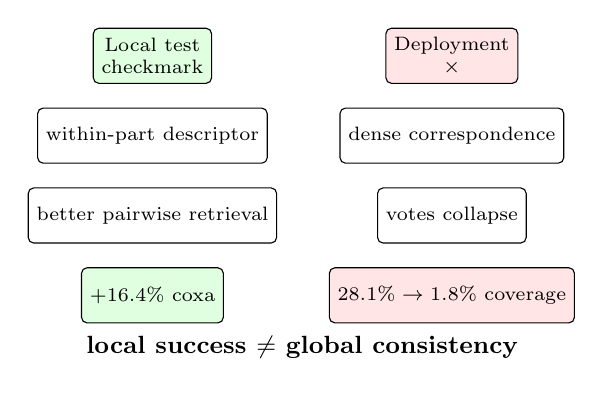
\begin{tikzpicture}[every node/.style={font=\scriptsize},
 n/.style={draw,rounded corners=2pt,minimum height=7mm,align=center,fill=white,inner sep=3pt}]
\node[n,fill=green!12] (a) {Local test\\checkmark};
\node[n,below=3mm of a] (a2) {within-part descriptor};
\node[n,below=3mm of a2] (a3) {better pairwise retrieval};
\node[n,below=3mm of a3,fill=green!12] (a4) {$+16.4\%$ coxa};
\node[n,right=22mm of a,fill=red!10] (b) {Deployment\\$\times$};
\node[n,below=3mm of b] (b2) {dense correspondence};
\node[n,below=3mm of b2] (b3) {votes collapse};
\node[n,below=3mm of b3,fill=red!10] (b4) {$28.1\%\to1.8\%$ coverage};
\node[below=4mm of $(a4)!0.5!(b4)$,font=\small\bfseries] {local success $\neq$ global consistency};
\end{tikzpicture}
\caption{The same descriptor, evaluated at two levels of abstraction. Strong
local (pairwise) retrieval does not imply a usable dense correspondence
field.}
\label{fig:local-vs-global}
\end{figure}

\begin{investigation}{I15}{Does strong pairwise retrieval accuracy translate
into a usable, dense correspondence field at deployment?}
\invQuestion{Deployed as a dense, whole-mesh correspondence mechanism rather
than evaluated pairwise at one joint, does the within-part descriptor still
outperform the existing geometric baseline?}
\invMethod{Full-mesh deployment benchmark across 48 specimens, learned
descriptor vs.\ geometric nearest-point baseline; a follow-up analysis
isolating how much of any gap is attributable to differences in the
candidate point set each method was allowed to match against, versus the
descriptor's votes themselves.}
\invResult{The learned descriptor performs \emph{worse} at deployment scale.
Candidate-set differences account for only about $2.9\%$ of the observed
gap, against an overall gap of roughly $145\%$; at the coxa specifically,
surface coverage collapses from $28.1\%$ under the geometric baseline to
$1.8\%$ under the learned descriptor.}
\invVerdict{REJECT}{The learned votes collapse onto a small subset of
points instead of producing a dense, globally consistent field across the
whole mesh. Pairwise retrieval accuracy at a single joint (Investigation~I14) is not
the same property as dense, globally consistent correspondence across an
entire specimen, and the two must be evaluated separately rather than
assumed to track each other.}
\end{investigation}

Read together, these four steps identify a specific, narrow gap rather than
a blanket failure of learning: local, within-part descriptors carry real
information (Investigation~I14) that geometric nearest-matching does not,
but turning that local signal into a dense, mesh-wide correspondence
field (global consistency, not just local accuracy) is an unsolved
engineering problem in its own right (Investigation~I15), and is the
concrete direction this report's outlook (Chapter~\ref{ch:conclusion})
recommends pursuing further.


\subsection*{Counterfactual diagnosis}
\section{Counterfactual bottleneck analysis}
\label{sec:oracle}

Every experiment so far asks \emph{can an intervention make the system
better?} An \term{oracle intervention} asks a different, more powerful
question: \emph{if this one piece of information were solved exactly, how
much of the failure would remain?} The fitter is supplied, at inference,
with the correct answer to exactly one sub-question (information it could
not obtain on real data), and the residual error localises the bottleneck
causally, without proposing a deployable fix. Two oracles were run on the
synthetic corpus, where ground truth is exact, escalating in how much
information is supplied.

\begin{center}
\small
\begin{tabular}{@{}p{0.17\linewidth}p{0.20\linewidth}p{0.30\linewidth}p{0.20\linewidth}@{}}
\toprule
\textbf{Oracle} & \textbf{Information supplied} & \textbf{What remains} & \textbf{Evidence} \\
\midrule
Regional identity & ``which structure is this?'' & Localisation error inside
  the correct structure & Leg accuracy $0.867\to0.937$ (\F{F3}) \\
Dense correspondence & ``where exactly, for every vertex?'' & Objective,
  deformation and trajectory effects, even with correspondence solved &
  Residual error persists \\
Expert joints (\S\ref{sec:skeleton-underdetermined}) & ``where is the true
  skeleton?'' & Incomplete propagation to unsupervised regions &
  $25.1\%\to17.4\%$ WL, leave-one-region-out null (\F{F6}) \\
\bottomrule
\end{tabular}
\end{center}

\textbf{Regional identity.} Every target point is labelled with the region it
truly belongs to (which leg, which body segment), leaving the optimiser to
decide only where \emph{within} that region the point sits. Leg accuracy
improves from $0.867$ to $0.937$: a real but partial recovery. A large share
of correspondence error survives even when ``which structure is this?'' is
answered perfectly, so the harder remaining question is \emph{where within
the structure} a point belongs: regional identity and within-region
localisation are distinct problems (\F{F3}).

\textbf{Dense correspondence.} A second oracle supplies near-exact per-vertex
correspondence, including at very high weight against the rest of the
objective. Residual error remains here too: the objective's other terms, the
deformation freedom of \S\ref{sec:deformation-freedom}, and the optimisation
trajectory continue to limit the fit even when correspondence is no longer
the constraint. This rules out the simplest reading of this report's central
theme, that correspondence is the \emph{only} missing ingredient, and
locates the problem in an interaction between correspondence, objective,
trajectory and deformation. A third, real-data oracle along the same logic
(supplying expert joint locations) is reported in
\S\ref{sec:skeleton-underdetermined}, where the same escalating pattern holds:
more information supplied recovers more accuracy, but does not propagate
beyond where it is supplied.


\chapter{Mechanistic Analysis of Registration Recoverability}
\label{ch:diagnostics}

% One file per section — edit independently under chapters/05_diagnostics/.
\section{One bad fit, many candidate causes}

A single failed registration (a smooth mass instead of an ant, as in
Chapter~\ref{ch:introduction}) can originate at any of six points in the
pipeline of Chapter~\ref{ch:pipeline}, and diagnosing it requires asking a
different question at each one (Figure~\ref{fig:one-bad-fit}): what evidence
is actually available in the scan; which anatomical structure a given region
of the template is meant to represent; what pose the model currently
assumes; which target point a given vertex should correspond to; whether the
model has enough freedom that a wrong correspondence can still be hidden
behind a locally plausible surface; and whether the optimiser can actually
reach the solution that scores best, even when one exists. The rest of this
chapter answers each of these questions in turn, using the synthetic
correspondence instrument built in \S\ref{sec:synthetic-instrument} as the
common measuring stick.

\begin{figure}[!htb]
\centering
\includegraphics[width=0.55\linewidth]{figures/fig_one_bad_fit_wheel.jpg}
\caption{A bad fit is rarely attributable to a single cause. The six axes
investigated in this chapter interact, and an intervention aimed at one can
leave the anatomical failure it was meant to fix untouched (Chapter~\ref{ch:interventions}).}
\label{fig:one-bad-fit}
\end{figure}

Section~\ref{sec:three-failure-modes} closes the chapter with three
concrete failure modes that recur across the diagnostics below, each
surprising relative to the intuitive fix it might suggest.

\section{The synthetic correspondence instrument}
\label{sec:synthetic-instrument}

No measurement of correspondence, as distinct from surface coverage, existed
in the pipeline before this internship. One was built from synthetic data
generated by the model itself: parameters $(\bm\beta, \bm\theta)$ are sampled
from the model's own learned distributions, the template is posed
accordingly, the result is exported as an anonymous mesh, optionally
degraded with noise, holes, or partial occlusion to resemble real scan
artefacts, and passed back through the fitter exactly as a real specimen
would be. Because the mesh originates from the model, the true identity of
every vertex is known by construction, so per-vertex correspondence error is
directly measurable rather than inferred indirectly from surface distance.
This instrument underlies every diagnostic in the remainder of this chapter.

\begin{investigation}{I1}{Is correspondence error a part-identity problem or a localisation problem?}
\invQuestion{When a vertex lands in the wrong place, would telling the
optimiser which anatomical region it belongs to remove most of the error?}
\invMethod{Round-trip fits of synthetic specimens with known vertex identity,
comparing the default fit against a fit given the correct \emph{regional
identity} of every target point (a counterfactual, or \emph{oracle},
intervention; \S\ref{sec:oracle}).}
\invResult{Leg accuracy improves from $0.867$ to $0.937$: a real but partial
recovery. Substantial error remains \emph{inside} correctly identified
structures.}
\invVerdict{DIAGNOSTIC}{Regional identity and within-region localisation are
separate problems, and fixes aimed only at part discrimination (segmentation
refinements, SDF-style descriptors) address only the first. This is a
causal-bottleneck finding, not a shipped intervention: no algorithm here is
adopted into the pipeline. Recorded as \F{F3}. An earlier percentage for this
split was derived under a reference later found to be invalid (\F{F7}) and is
not reported.}
\end{investigation}

\section{Can the input be trusted? A controlled null result}
\label{sec:prep-null}

\begin{figure}[!htb]
\centering
\includegraphics[width=0.6\linewidth]{figures/fig_before_registration.jpg}
\caption{Raw scans before registration: holes, self-intersections and
missing surface at exactly the structures of greatest anatomical interest:
the visual evidence motivating the brief's preprocessing-first
hypothesis.}
\label{fig:before-registration}
\end{figure}

The internship brief's implicit hypothesis was that input mesh quality was
the dominant bottleneck (Figure~\ref{fig:before-registration}). The first
weeks were spent building a unified preprocessing pipeline with explicit
diagnostics and quality classification, retained in the delivered system
because its outputs make later fitting decisions auditable.

\begin{investigation}{I2}{Does cleaner input produce more accurate registration?}
\invQuestion{Holding the registration stage fixed, does the rebuilt
preprocessing pipeline improve fit accuracy over the existing one?}
\invMethod{Head-to-head mean Chamfer distance across a matched specimen set,
new pipeline vs.\ existing pipeline, registration stage identical.}
\invResult{$0.000771$ (new) vs.\ $0.000737$ (existing), under five
percent apart, nominally \emph{favouring} the existing pipeline, and far too
small to account for the correspondence gap characterised in
\S\ref{sec:synthetic-instrument}.}
\invVerdict{REJECT}{Topology improved substantially (\S3.3) without moving
this surface metric, so mesh conditioning alone does not explain the
correspondence failures under investigation. This comparison uses Chamfer
distance as a coverage check, not an anatomical-correctness check
(\F{F1} shows the latter is unreliable); the claim is deliberately limited to
what Chamfer distance can support (coverage did not change), and
motivated testing whether the limitation lay downstream of mesh conditioning
instead. Recorded as \F{F2}.}
\end{investigation}

A clear improvement here would have justified further investment in
preprocessing; instead, the comparison ruled out mesh quality as the
dominant explanation and reframed the central question of the internship
from \emph{how clean is the input} to \emph{what determines whether the
optimiser finds the right correspondence at all}: the question the rest
of this chapter answers.

\section{Can geometric agreement be trusted?}
\label{sec:geometric-agreement}

\begin{figure}[!htb]
\centering
\includegraphics[width=0.58\linewidth]{figures/fig_geometric_agreement.jpg}
\caption{Removing anatomical (rotation-limit) constraints from the objective
moves surface distance and skeleton accuracy in \emph{opposite} directions:
the fit looks better by the metric the optimiser sees, and is worse by the
metric that matters. Skeleton overlay: blue, with anatomical constraints
active.}
\label{fig:geometric-agreement}
\end{figure}

\begin{investigation}{I3}{Is surface agreement a safe proxy for anatomical correctness?}
\invQuestion{If a fit's Chamfer distance improves, has the underlying
skeleton also become more accurate?}
\invMethod{Same specimen set, anatomical rotation-limit constraints toggled
on and off, Chamfer distance and joint-position error compared under each
configuration.}
\invResult{Removing constraints yields $0.45\times$ the Chamfer distance (a
closer surface) but $1.25\times$ the joint error (a worse skeleton): the
fit that scores better on the objective's own terms is the anatomically
worse one.}
\invVerdict{REJECT}{Surface-proximity metrics alone cannot adjudicate fit
quality. Confirms \F{F1}, independently of the rotation-probe and
10-specimen batch results referenced in the findings ledger
(\S\ref{sec:ledger}), and is the direct motivation for the two-tier
evaluation suite of \S\ref{sec:eval-suite}.}
\end{investigation}

The mechanism is not subtle once stated: every term in the registration
objective (\S\ref{sec:registration}) is a function of the two surfaces, and
none of them is a function of which point on the template surface is
supposed to represent which point on the target. A lower value of
$\mathcal{L}_{\mathrm{chamfer}}$ certifies that the fitted mesh covers the
target; it does not certify that vertex $i$ has landed on the anatomical
locus vertex $i$ is defined to represent. \S\ref{sec:skeleton-underdetermined}
traces this observation to a specific, structural property of the objective.

\section{Can the model find the right articulation?}
\label{sec:articulation}

\begin{figure}[!htb]
\centering
\includegraphics[width=0.62\linewidth]{figures/fig_articulation_flow.jpg}
\caption{A pose error near the body (proximal) propagates downstream through
the kinematic chain, so the vertex most likely to end up mis-corresponded is
not the one where the error originated but everything distal to it.}
\label{fig:articulation-flow}
\end{figure}

\begin{figure}[!htb]
\centering
\includegraphics[width=0.5\linewidth]{figures/fig_articulation_bars.jpg}
\caption{Leg accuracy for the same total amount of pose error, placed at
different points along the kinematic chain. Moving an identical error budget
from the tip (distal) to the base (proximal) of the leg is the difference
between a recoverable fit (0.94) and a badly broken one (0.77).}
\label{fig:articulation-bars}
\end{figure}

\begin{investigation}{I4}{Is initialisation sensitivity uniform along the kinematic chain?}
\invQuestion{Does starting the optimiser from the ground-truth pose recover
the accuracy lost under default initialisation, uniformly across the
kinematic chain?}
\invMethod{Ground-truth-initialised vs.\ zero-initialised fits, per joint,
on the synthetic corpus; a matched pose-error-placement sweep
(Figure~\ref{fig:articulation-bars}) isolating the effect of \emph{where}
along the chain a fixed error budget is placed.}
\invResult{For the distal chain, ground-truth initialisation recovers most
of the lost accuracy: pretarsus improves twelvefold ($0.1717\to0.0140$),
tibia eightfold, tarsus and femur both significant at $p<0.002$. The coxa is
the exception: ground-truth initialisation there is statistically
indistinguishable from a default start ($0.4204$ vs.\ $0.4114$, $p=0.47$),
and the optimiser measurably walks the coxa \emph{away} from the correct
pose it is handed, by a mean of $0.222$\,rad.}
\invVerdict{HOLD}{Initialisation sensitivity is anatomically heterogeneous
(\F{F4}): a better starting point strongly helps the distal chain, but at the
coxa it cannot help, because the optimum reached from any start is not the
correct pose. Two regimes, not one.}
\end{investigation}

The coxa result is the more consequential of the two, because it cannot be
fixed by improving the initialisation network of \S\ref{sec:init-stage}: no
matter how good the starting guess, the optimiser will walk away from it.
\S\ref{sec:skeleton-underdetermined} pursues this to its mechanism.

\section{Can deformation be allowed to fix everything?}
\label{sec:deformation-freedom}

\begin{figure}[!htb]
\centering
\includegraphics[width=0.58\linewidth]{figures/fig_deformation_shortcut.jpg}
\caption{What happens when the model has enough freedom to make the surface
look right regardless of pose. Left: a structured correction, achieved
through the model's own pose and shape parameters. Right: the same visual
improvement achieved by free per-vertex deformation, which bends the leg
rather than re-posing the joint.}
\label{fig:deformation-shortcut}
\end{figure}

The registration objective includes free per-vertex deformation terms,
bounded only by edge-length and Laplacian regularisation
(\S\ref{sec:registration}), because the model's fixed shape space cannot by
itself represent every idiosyncrasy of a real specimen. This freedom is
also, mechanically, an escape hatch: a joint that is posed incorrectly can
be visually corrected either by rotating it to the right angle, or by
bending the mesh around a wrong angle until the surface distance term is
satisfied anyway (Figure~\ref{fig:deformation-shortcut}). The two solutions
can be nearly indistinguishable by $\mathcal{L}_{\mathrm{chamfer}}$ while
being anatomically unrelated: only the first preserves the correspondence
that makes the fit usable for measurement (Chapter~\ref{ch:validation}).

This is the same mechanism as \F{F1} (\S\ref{sec:geometric-agreement}),
observed at the level of a single joint rather than a whole specimen, and it
is why deformation cost is treated in the delivered recipe as a
\emph{regularising} penalty rather than a free parameter: neither an
unbounded deformation budget nor a frozen one is correct, because the
optimum that best serves anatomical correctness sits in between the two
(\S\ref{sec:three-failure-modes}).

\section{Objective under-determination of skeletal position}
\label{sec:skeleton-underdetermined}

The coxa result in \S\ref{sec:articulation} was pursued to a mechanism
rather than left as an observation; doing so honestly first required
checking the ground truth being pursued against. An early set of expert
joint annotations was recorded in Blender's internal coordinate convention,
one axis permutation, $(x,y,z)\mapsto(x,z,-y)$, away from the convention
used by the scan meshes those annotations were meant to describe; a
derived skeleton reference file inherited the same mismatch. Every
conclusion drawn against that reference in the project's first analysis
pass, including an apparent $42.7\%$ production skeleton error, was
invalidated once this was found, and discarded. This is reported as a
technical result in its own right (\F{F7}), not a caveat: catching a
ground-truth defect before it propagates into a project's headline claims
is exactly the discipline a registration pipeline needs.

\begin{investigation}{I5}{Does the objective actually constrain skeleton
position, once the ground truth used to check it is trustworthy?}
\invQuestion{Is there a solution, reachable within the model's own shape
budget, that is substantially more anatomically accurate than production's,
and if so, why does the optimiser not find it?}
\invMethod{The corrected \term{Joint Alignment Benchmark}: eleven
expert-annotated specimens, re-registered against the mesh coordinate
convention to a residual of $7\times10^{-8}$, frozen and hash-verified,
yielding 396 fits under a fixed protocol. Expert joint targets are supplied
directly during fitting and compared against the unsupervised production
fit; a systematic single-factor sweep re-tests every existing objective term
in isolation; a leave-one-region-out variant withholds expert targets for
one anatomical region at a time.}
\invResult{Production skeleton error is $25.1\%$ of Weber's length (95\% CI
$17.5$--$44.8\%$). Supplying expert joint targets during fitting reduces
this to $17.4\%$ ($10$ of $11$ specimens improved). The single-factor sweep
found no individual existing objective term that reliably improved joint
alignment on its own (Friedman test, $p=.011$, with the unmodified
production configuration retaining the best mean rank across variants).
Leave-one-region-out supervision does not propagate: for every held-out
region, the confidence interval for improvement included zero.}
\invVerdict{REJECT}{The production objective contains no explicit
observation term for joint location. Its surface terms constrain the
skeleton only indirectly, through the skinned surface it produces, and do
not distinguish all anatomically different latent configurations that yield
similar surfaces. No single existing term, reweighted or removed, fixes this
reliably, and supervision supplied for one region does not propagate to
another. Recorded as \F{F6}; it also explains why reweighting existing terms
(\S\ref{sec:eliminated}) returned null results.}
\end{investigation}

The error this benchmark measures is itself structured rather than uniform.
Proximal joints are recovered far more reliably than distal ones:
coxae at $11.6\%$ of Weber's length, trochanter/femur at $12.9\%$, while
the body axis, mandibles, antennae, and tibia/tarsus segments range from
$24\%$ to over $56\%$ (Table~\ref{tab:regional-error}). A log-scale variance
decomposition attributes far more of the spread in this benchmark to
\emph{which joint} and \emph{which specimen} than to \emph{which random
seed} the optimiser started from.

\begin{table}[!htb]
\centering
\caption{Regional skeleton error (\% of Weber's length) on the corrected
benchmark, and the log-scale variance decomposition across the same fits.}
\label{tab:regional-error}
\begin{tabular}{@{}lc@{\hspace{2.5em}}lc@{}}
\toprule
\textbf{Anatomical region} & \textbf{Error} & \textbf{Variance source} & \textbf{Share} \\
\midrule
Coxae               & 11.6\% & Which joint          & 0.36 \\
Trochanter / femur   & 12.9\% & Which specimen       & 0.17 \\
Body axis            & 24.1\% & Optimiser random seed & 0.02 \\
Mandibles            & 42.8\% & & \\
Antennae             & 54.9\% & & \\
Tibia / tarsus       & 56.3\% & & \\
\bottomrule
\end{tabular}
\end{table}

Registration failure is therefore anatomically structured, not attributable
to optimiser luck (\F{F8}): a fit that happens to land badly is far more
likely to have landed on a hard joint or a hard specimen than to have simply
been unlucky in its random initialisation.

\section{A defect in the staged fitting schedule}
\label{sec:staged}

The registration stage (\S\ref{sec:registration}) runs as four sequential
stages (initialisation, posing/transforming, coarse vertex deform, fine
vertex deform), and the audit around \F{F4} and \F{F6} also exposed
a defect in how this schedule allocates iterations: pose was held fixed for
2000 of the refinement stage's 2400 iterations, with only the first 400
free to adjust joint rotation before vertex deformation took over. Because
Chamfer distance descends smoothly regardless of when pose freezes relative
to deformation, this defect produced no visible signature in the loss curve
and survived undetected until this investigation. A rebuilt schedule
widening the pose-adjustable window was tested against the stock schedule on
the full integrity-metric suite of \S\ref{sec:eval-suite}: it improves
nearly every metric measured, at no additional computational cost, and was
shipped into the delivered recipe. This is a second, independent instance of
the pattern in \F{F1}: the objective's own value is not a reliable signal
for whether the fitting procedure that produced it was sound, caught only
because integrity metrics, not surface distance alone, were checked.

\section{Three failure modes}
\label{sec:three-failure-modes}

The diagnostics above converge on three failure modes, each of which
contradicts a natural first guess at how to fix it:

\begin{enumerate}
\item \textbf{Self-generated targets still fail to recover.} With exact
correspondence and zero noise, recovery still breaks (\S\ref{sec:articulation}):
the failure is not solely a data-quality artefact that a cleaner target
would remove.
\item \textbf{Anatomical supervision does not generalise spatially.} Ground
truth supplied everywhere else produces no detectable improvement in a
held-out region: supervision at one location does not transfer to
another the way a smooth prior might suggest.
\item \textbf{Deformation cost functions as a regulariser, not a hard
constraint.} Neither fully free nor fully frozen deformation is correct
(\S\ref{sec:deformation-freedom}); the anatomically best-behaved optimum sits
strictly between the two extremes.
\end{enumerate}

Together with \F{F1}--\F{F6}, these three failure modes set the criteria
against which every candidate intervention in Chapter~\ref{ch:interventions}
is judged: not whether it improves the statistic it directly targets, but
whether it moves the anatomical outcome that statistic is meant to serve.


\chapter{Comparative Evaluation of Interventions}
\label{ch:interventions}

% One file per section — edit independently under chapters/06_interventions/.
Chapter~\ref{ch:diagnostics} localised the bottleneck; this chapter reports
what was done about it. The remainder of the internship proceeded by
systematic elimination: every candidate intervention was tested against a
criterion registered \emph{before} the experiment was run, so that a
favourable-looking result could not be reinterpreted after the fact. Each
candidate is reported here with the outcome that criterion produced:
\textsc{adopt}, \textsc{reject}, or \textsc{hold}; and, where the
evidence is informative beyond the pass/fail outcome, the residual signal
it left behind.

\section{A multi-level evaluation protocol}
\label{sec:eval-suite}

\F{F1} showed that surface-proximity metrics can reward an anatomically worse
fit. A direct adversarial test sharpens this: deliberately snapping distal
vertices onto the nearest target surface improves a per-part distance metric
by $53\%$ while edge-length distortion rises $7.5$-fold. A metric that a
targeted attack can improve by damaging the mesh cannot be the sole judge of
a fit. The protocol therefore has three evidence levels, always used
together:

\begin{center}
\begin{tabular}{@{}p{0.18\linewidth}p{0.34\linewidth}p{0.36\linewidth}@{}}
\toprule
\textbf{Level} & \textbf{Metrics} & \textbf{Question answered} \\
\midrule
1. Surface proximity & Chamfer, F-score, Hausdorff, per-part variants &
  Does the fitted mesh cover the target? \\
2. Target-independent integrity & Edge-length distortion, Laplacian /
  as-rigid-as-possible deviation~\cite{arap}, normal consistency &
  Was that coverage bought by damaging the mesh? \\
3. Anatomical ground truth & Synthetic vertex-identity error
  (\S\ref{sec:synthetic-instrument}); expert joint error on the corrected
  benchmark (\S\ref{sec:skeleton-underdetermined}) &
  Is vertex $i$ on the anatomical locus it represents? \\
\bottomrule
\end{tabular}
\end{center}

An intervention is adopted only if it does not degrade levels 1--2 and is
checked at level 3 wherever ground truth exists.

\section{Retained and qualified interventions}
\label{sec:retained}

Each intervention is recorded as hypothesis $\rightarrow$ expected mechanism
$\rightarrow$ proxy metric $\rightarrow$ anatomical metric $\rightarrow$
outcome, so that a proxy improvement cannot be mistaken for a mechanism
improvement (\S\ref{sec:methodological-discipline}).

\begin{center}
\small
\begin{tabular}{@{}p{0.16\linewidth}p{0.22\linewidth}p{0.22\linewidth}p{0.30\linewidth}@{}}
\toprule
\textbf{Intervention} & \textbf{Mechanism expected} & \textbf{Proxy result} & \textbf{Anatomical outcome} \\
\midrule
Joint rotation limits as a fitting prior & Remove impossible poses on the one
  path that had no angular constraint & Fewer implausible poses &
  Plausible, not correct: correspondence unresolved (\F{F1}). Integrated into
  the production fitting path. \\
Staged schedule with pose kept free longer & Fix pose frozen for 2000 of 2400
  refinement iterations (\S\ref{sec:staged}) & Nearly all integrity metrics
  improve, no extra cost & Consistent with the integrity gains; shipped into
  the production recipe. \\
Per-joint scale barrier & Curb anterior scale outliers that distort head,
  mandible, antenna groups & Outlier statistic reduced substantially in
  controlled experiments & Intended anterior morphology did \emph{not}
  measurably improve; retained as a numerical stabiliser rather than a
  solved anatomical correction (below). \\
\bottomrule
\end{tabular}
\end{center}

\textbf{The scale barrier is a qualified intervention.} It was implemented
and evaluated as a targeted regularizer. It moved its own proxy, the
scale-outlier statistic, but a separate test of the anatomical mechanism it
was meant to correct, the deformation ratio between the head, mandible and
antenna groups and the thorax, found none of the three ratios moving
significantly toward its expected value. It is retained as a numerical
stabiliser, not as a solved anatomical defect, and the defect remains open
(Chapter~\ref{ch:conclusion}). A downstream check on a small existing
benchmark was directional only and underpowered; no corpus-scale validation
is claimed here.

\section{Eliminated candidates}
\label{sec:eliminated}

\begin{center}
\begin{tabular}{@{}p{0.34\linewidth}p{0.52\linewidth}@{}}
\toprule
\textbf{Candidate} & \textbf{Reason for rejection} \\
\midrule
Part-level segmentation refinements (SDF-based~\cite{sdf} and other
  intrinsic geometric descriptors) & Address part identity only;
  \F{F3} shows that correct regional identity recovers just part of the error \\
Reweighting existing objective terms (surface, edge, normal, Laplacian,
  offset, symmetry, midline) & None observes joint location explicitly
  (\F{F6}); reweighting a term that does not measure the missing quantity
  cannot recover it; single-factor sweep found no reliable gain \\
Partition-based split of the objective (anterior/posterior) & Null result on
  the anterior deformation statistic it targeted \\
Correspondence-confidence probe using an untrained auxiliary network & Its
  apparent failure pattern was traced to the network silently failing to
  load its pretrained weights, not to a property of the correspondence
  problem itself \\
An additional shape-prior penalty term & Quadrupled the cost it was meant to
  control, rather than reducing it \\
\bottomrule
\end{tabular}
\end{center}

Two rejected candidates left a positive residual worth recording rather than
discarding outright. \textbf{Extrinsic learned image features} (descriptors
trained on image context rather than intrinsic mesh geometry) carried real
anatomical correspondence signal where every intrinsic geometric descriptor
tested, including the Shape Diameter Function~\cite{sdf}, carried
none. A \textbf{context-trained descriptor} specifically outperformed rigid
nearest-surface matching at the coxa, the joint at which \F{F4} shows
initialisation does not help. Neither candidate was deployable
within the internship's timeframe, but together they identify extrinsic
learned features as the one candidate family not bounded by the within-part
within-part localisation ceiling in \F{F3}, and therefore the most promising
direction for future work on this problem (Chapter~\ref{ch:conclusion}).

\section{Proxy-to-mechanism validation}
\label{sec:methodological-discipline}

One principle recurs across every intervention above, and is applied to the
report's own claims. For each intervention two questions are asked
separately: (i) \emph{did it change its intended proxy?} and (ii) \emph{did
the anatomical mechanism the proxy stands for actually improve?} The
investigation repeatedly found $\text{proxy}\uparrow \not\Rightarrow
\text{mechanism}\uparrow$: lower Chamfer with a worse skeleton (\F{F1}), a
scale statistic that improved without the anterior morphology improving,
and a validation instrument whose own synthetic estimate did not survive
expert ground truth (\S\ref{sec:reliability}). This is a general lesson of
optimisation and scientific machine learning: an objective is a proxy for
the property one cares about, and is treated here as a design rule:
every result is reported with the level of evidence that supports it
(Table~\ref{tab:evidence}).


\chapter{From registration to measurement to biology}
\label{ch:validation}

% One file per section — edit independently under chapters/07_validation/.
\section{An independent anatomical ground truth}

The synthetic instrument of \S\ref{sec:synthetic-instrument} answers whether
the pipeline can recover a correspondence it generated itself. It cannot, by
construction, answer whether the pipeline is right about a \emph{real}
specimen. Closing that gap required an independent reference the pipeline
had no part in producing.

\begin{figure}[!htb]
\centering
\includegraphics[width=0.55\linewidth]{figures/fig_ground_truth_annotation.jpg}
\caption{Manual 3D joint annotation as an independent reference: an expert
places joints directly on the scan, with identity known by construction,
against which the model's inferred correspondence can be verified rather
than merely inspected.}
\label{fig:ground-truth-annotation}
\end{figure}

\begin{figure}[!htb]
\centering
\includegraphics[width=0.6\linewidth]{figures/fig_landmarks_structured.jpg}
\caption{Expert-annotated joints across four specimens. Reliability is not
uniform across the body: it is structured, concentrated proximally, and
degrades toward the distal leg and antenna segments, consistent with the
sampling deficit in \F{F5}.}
\label{fig:landmarks-structured}
\end{figure}

Manual 3D joint annotation (Figure~\ref{fig:ground-truth-annotation})
supplies this reference. Evaluated against it, the delivered fits are close
to unbiased across every anatomical block, but, as \S\ref{sec:reliability}
details, do not reliably \emph{rank} specimens against one another. This
is the first accuracy statement in the project grounded in expert-verified
data rather than the pipeline's own synthetic ground truth, and it is not
uniformly favourable: it delimits precisely which claims the current fits
support (Figure~\ref{fig:landmarks-structured}).

\section{When does a parameter become a measurement?}
\label{sec:measurement}

\begin{figure}[!htb]
\centering
\includegraphics[width=0.6\linewidth]{figures/fig_parameter_measurement.jpg}
\caption{Head width read directly from 20 fitted \emph{Atta} workers against
an independent physical reference measurement.}
\label{fig:parameter-measurement}
\end{figure}

A fitted parametric model is not an end in itself; it is an instrument.
Once every specimen occupies the shared coordinate system of
\S\ref{sec:pipeline-overview}, quantities entomologists currently extract
manually under a microscope (head width, body length, appendage
proportions) become extractable automatically and at population scale,
\emph{provided} the extracted numbers agree with what a caliper would
report. This is the check that closes the chain this report has followed
throughout: \textbf{registration} $\rightarrow$ \textbf{measurement}
$\rightarrow$ \textbf{biological value}.

On a 20-specimen \emph{Atta} worker corpus, joint positions recovered
directly from the fitted model reach a median error of $1.05\%$ of Weber's
length against expert reference measurements, with $96\%$ of joints within
$5\%$, consistent with the coxa-and-body-axis end of the regional error
profile in Table~\ref{tab:regional-error}, on a corpus with less of the
distal-appendage difficulty that dominates the harder end of that table.
Two independent allometric relationships (head width against body
length, and head width against body mass) reproduce published reference
slopes closely ($1.189$ vs.\ $1.235$, and $0.380$ vs.\ $0.395$
respectively), with $R^2$ between $0.987$ and $0.993$. Figure~\ref{fig:parameter-measurement}
shows the same agreement directly, in absolute units: a mean difference of
$4\%$ between SMILify-derived and independently measured head width.

Two further checks were made before treating this agreement as settled. The
first compared two competing definitions of ``head width'': one read from
the model's own joint-derived reference points, the other from an
alternative purely geometric definition. The joint-derived definition showed
a smaller bias against the physical reference ($-0.13\%$) than the
geometric one ($+2.22\%$), so it is the definition used throughout this
report. The second check is a methodological one worth stating generally:
raw agreement in millimetres can partly be inherited from shared
whole-body-length scaling rather than from an independently accurate
measurement, so a \emph{dimensionless} ratio such as head width over body
length is a more informative validation target than absolute agreement
alone, and is reported alongside it here for that reason.

\section{Population-level signal: a provisional result}
\label{sec:genus}

Whether traits read from fitted models carry biological signal in aggregate
was tested by \emph{lot-blind nearest-neighbour classification}: each
specimen is assigned the genus of its nearest neighbour in trait space,
excluding specimens from the same collection lot so that nest-mates cannot
leak the answer, and the resulting accuracy is compared with a
\emph{permutation null} in which genus labels are shuffled. An earlier
full-corpus analysis reported accuracy well above this null. That corpus
could not be re-executed in the final computing environment, and the only
available re-check (22 specimens, 9 genera) was underpowered and is
directional at most. The result is therefore reported as \textbf{provisional}
and deliberately excluded from this report's headline claims; the protocol
details a reader would need to audit it (lot definition, number of
permutations, treatment of rare genera, scale normalisation, trait selection
before classification) must accompany the run artifacts before it is cited
as validated (Table~\ref{tab:evidence}).

What the design does show is why aggregate signal and individual reliability
are compatible (\S\ref{sec:scale-dependence}): averaging over many specimens
and vertices suppresses within-part localisation noise (\F{F3}), whereas the
rank of any single specimen against another does not enjoy that protection.

\section{What the fits can, and cannot, be trusted for}
\label{sec:reliability}

\begin{investigation}{I8}{Do the delivered fits rank individual specimens
correctly, or only describe them correctly on average?}
\invQuestion{Against expert-corrected joint annotations, how many
joint-derived features reliably distinguish one specimen from another?}
\invMethod{Correlation of 49 joint-derived features against expert ground
truth; a parallel comparison of surface-landmark-derived traits against
rig-joint-derived traits at genus level.}
\invResult{Of 49 joint-derived features, only one reaches a correlation of
$0.5$ with expert ground truth. Registration of an independent
ethanol-preserved worker corpus sits at a measurable noise floor, at which
conspecific nest-mates are only $7\%$ closer than unrelated specimens; the
traits that fail the reliability threshold are precisely the distal leg and
antenna segment lengths that \F{F5} identified as under-sampled. On the same
fits, anatomical landmarks placed directly on the mesh surface carry more
genus-level signal than rig-derived joint distances in the earlier (provisional, \S\ref{sec:genus}) analysis, since a
rig joint is a rotation pivot rather than an anatomically defined point.}
\invVerdict{HOLD}{Population-level aggregates over many specimens are
supported by the current fits; per-specimen and comparative claims from
joint-derived measurements are not. For this reason the delivered
measurement layer reports surface-derived traits rather than rig lengths.}
\end{investigation}

A further consequence concerns the validation instrument itself, not only
the fitting pipeline: the project's own synthetic reliability estimate did
not survive contact with this expert ground truth. This is a second, more
consequential instance of the metric-versus-mechanism pattern in
\S\ref{sec:methodological-discipline}, here applied to the validation
instrument rather than to a fitting intervention, and it is the reason
this report treats expert-verified ground truth, wherever available, as the
higher-authority reference throughout.

\section{Validity is scale-dependent}
\label{sec:scale-dependence}

Taken together, the results of this chapter show that ``the registration is
valid'' is not one claim but four, holding at different scales and by
different evidence:

\begin{center}
\small
\begin{tabular}{@{}p{0.19\linewidth}p{0.36\linewidth}p{0.33\linewidth}@{}}
\toprule
\textbf{Level} & \textbf{Question} & \textbf{Evidence in this report} \\
\midrule
Surface correspondence & Are the two surfaces geometrically close? &
  Chamfer, F-score (misleading alone, \F{F1}) \\
Anatomical correspondence & Does model location $i$ mark the same structure
  across specimens? & Synthetic oracle, corrected expert benchmark
  (\F{F3}, \F{F6}) \\
Parametric correspondence & Do recovered $\bm\beta,\bm\theta$ mean the same
  thing across specimens? & Only partially established: 1 of 49
  joint-derived features reaches $r=0.5$ \\
Measurement validity & Does a derived measurement match an independent one? &
  Atta head width, allometric slopes (\S\ref{sec:measurement}) \\
\bottomrule
\end{tabular}
\end{center}

A model can therefore give accurate population-level and head-width
measurements while failing to preserve the individual-level correspondence
needed for specimen-by-specimen comparison of distal segment lengths. Both
statements are true, and each is supported only at its own level.

\section{Demonstrated headroom}
\label{sec:validation-headroom}

The expert-supervised fit introduced in \S\ref{sec:skeleton-underdetermined}
is the one result in this report that moves skeleton accuracy against
\emph{human ground truth}, rather than only against a self-consistency or
synthetic-corpus statistic: supplying expert joint targets during fitting
reduces skeleton error from production's $25.1\%$ of Weber's length to
$17.4\%$. This is reported as demonstrated headroom rather than a deployed
capability, because it depends on expert joint annotations unavailable at
inference time; supplying an equivalent signal automatically, from a learned
3D joint predictor, is the concrete engineering objective this result
motivates for the project's next phase (Chapter~\ref{ch:conclusion}).


\chapter{Discussion, limitations and outlook}
\label{ch:conclusion}

\section{Discussion}

\textbf{What the experiments collectively establish.} The internship began
by assuming input quality was the limit and found it was not (\F{F2}).
Surface proximity was then shown to be an unreliable proxy for anatomy
(\F{F1}); correspondence splits into identity and localisation (\F{F3});
initialisation matters for distal segments but not at the coxa (\F{F4});
and the objective has no explicit joint observation term (\F{F6}), so
anatomically different configurations can produce similar surfaces. Error is
structured by joint and specimen, not by seed (\F{F8}).

\textbf{Why this is a non-identifiability problem.} The scan supplies
surface geometry; the optimiser explicitly recovers shape, pose, scale and
deformation, and anatomical correspondence is an intended consequence of
those recovered parameters rather than an independently observed quantity.
Several latent configurations give geometrically similar surfaces, so the
surface observation does not uniquely determine the underlying anatomical
state: the inverse map is non-identifiable in the configurations tested here.
Each mechanism studied acts on that ambiguity: free deformation $\mathbf d$
can absorb a pose error (\S\ref{sec:deformation-freedom}); pointwise learned
votes can be locally right and globally inconsistent
(\S\ref{sec:learned-correspondence}), a mismatch between a pairwise
retrieval objective and a deployment problem that is really a globally
coupled assignment; and supervision at one place does not constrain another.

\textbf{Synthetic-to-real limits.} Learned components trained on synthetic
targets did not transfer at the trained perturbation regime
(\S\ref{sec:pointnet-init}), and the project's own synthetic reliability
estimate did not survive expert ground truth (\S\ref{sec:reliability}).

\textbf{Four distinctions.} Representability is not recoverability;
identity is not location; plausibility is not correspondence; fit quality is
not measurement validity. Each was the concrete reason a plausible
intervention failed. The central outcome is therefore not one configuration
but experimentally validated distinctions between geometric proximity,
anatomical correspondence, parameter recovery and measurement validity: a
diagnostic framework for SMILify and a design criterion for future
body-plan-agnostic models. A useful parametric representation is defined not
only by what it can represent, but by what anatomical meaning survives its
recovery from data. A reconstruction is not yet a phenotype.

\section{Evidence status of headline claims}

\begin{table}[!htb]
\centering
\caption{Evidence status. \emph{Validated}: completed, with artifacts.
\emph{Qualified}: proxy validated, mechanism unresolved.
\emph{Provisional}: obtained earlier, not reproducible in the final
environment.}
\label{tab:evidence}
\small
\begin{tabular}{@{}p{0.62\linewidth}p{0.28\linewidth}@{}}
\toprule
\textbf{Claim} & \textbf{Status} \\
\midrule
Corrected JAB: 11 specimens, 396 fits; production $25.1\%$ WL & Validated \\
Expert supervision $26.9\%\to17.4\%$ (10/11 improve); no propagation to
  held-out regions & Validated \\
Coordinate-frame correction (\F{F7}) & Validated \\
Surface vs.\ skeleton dissociation ($0.45\times$ / $1.25\times$) & Validated \\
Regional-identity oracle $0.867\to0.937$ & Validated (synthetic) \\
PointNet: synthetic gain, real-scan transfer failure & Validated \\
W3 within-part gain; W5 deployment collapse & Validated (controlled) \\
SDF: real-scan instance-separation failure & Validated \\
Scale barrier & Qualified: proxy only \\
Corpus-scale (838-specimen) barrier validation & Not claimed \\
Genus-level permutation-null result & Provisional \\
Functional maps, OT, canonical fields & Future work \\
\bottomrule
\end{tabular}
\end{table}

\begin{table}[!htb]
\centering
\caption{Master experiment table: each investigation's hypothesis, evidence,
and the interpretation the evidence supports.}
\small
\begin{tabular}{@{}p{0.05\linewidth}p{0.23\linewidth}p{0.14\linewidth}p{0.18\linewidth}p{0.30\linewidth}@{}}
\toprule
\textbf{ID} & \textbf{Hypothesis tested} & \textbf{Data} & \textbf{Result} & \textbf{Interpretation} \\
\midrule
I1 & Error is a part-identity problem & Synthetic & Oracle $0.867\to0.937$ &
  Identity and within-region localisation are distinct; the latter dominates \\
I2 & Preprocessing dominates recovery & Real & Chamfer tie despite better
  topology & Mesh conditioning alone does not explain the failure \\
I3 & Surface score tracks anatomy & Real, expert & $0.45\times$ / $1.25\times$
  & Surface proximity and anatomical correctness can move in opposite
  directions \\
I4 & Initialisation explains failure uniformly & Synthetic & Distal
  recovers, coxa does not & Sensitivity is anatomically heterogeneous, not
  uniform \\
I5 & Objective directly observes skeleton position & Expert real &
  $25.1\%\to17.4\%$ with supervision, no propagation & Skeleton position is
  constrained only indirectly; supervision does not generalise spatially \\
I11 & Learned initialisation transfers to real data & Synth./real & Fails at
  the trained perturbation regime & Consistent with synthetic-to-real
  distribution mismatch \\
I14 & A local descriptor carries correspondence signal & Synthetic &
  $+16.4\%$ held-out improvement & Local learned signal exists beyond raw
  geometry \\
I15 & That signal deploys as dense correspondence & Synth./real & Coverage
  collapse ($28.1\%\to1.8\%$) & Pairwise retrieval accuracy does not imply
  globally consistent correspondence \\
\bottomrule
\end{tabular}
\end{table}

\begin{figure}[!htb]
\centering
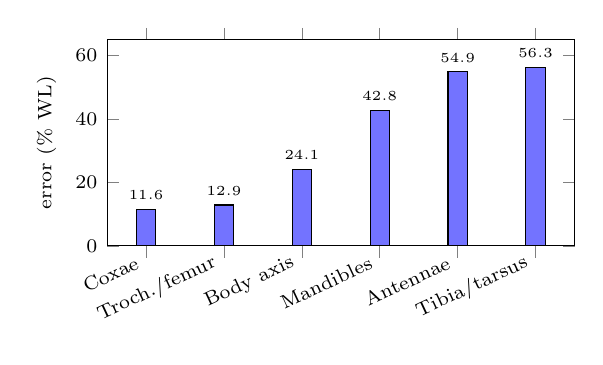
\begin{tikzpicture}
\begin{axis}[ybar,width=0.62\linewidth,height=4.2cm,bar width=7pt,ymin=0,ymax=65,
 symbolic x coords={Coxae,Troch./femur,Body axis,Mandibles,Antennae,Tibia/tarsus},
 xtick=data,x tick label style={rotate=25,anchor=east,font=\scriptsize},
 ylabel={error (\% WL)},ylabel style={font=\scriptsize},tick label style={font=\scriptsize},nodes near coords,
 every node near coord/.append style={font=\tiny}]
\addplot[fill=blue!55] coordinates {(Coxae,11.6)(Troch./femur,12.9)(Body axis,24.1)(Mandibles,42.8)(Antennae,54.9)(Tibia/tarsus,56.3)};
\end{axis}
\end{tikzpicture}
\hfill
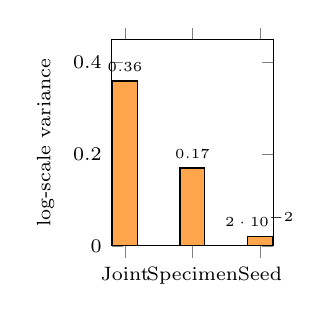
\begin{tikzpicture}
\begin{axis}[ybar,width=0.30\linewidth,height=4.2cm,bar width=9pt,ymin=0,ymax=0.45,
 symbolic x coords={Joint,Specimen,Seed},xtick=data,tick label style={font=\scriptsize},
 ylabel={log-scale variance},ylabel style={font=\scriptsize},nodes near coords,every node near coord/.append style={font=\tiny}]
\addplot[fill=orange!70] coordinates {(Joint,0.36)(Specimen,0.17)(Seed,0.02)};
\end{axis}
\end{tikzpicture}
\caption{Left: regional skeleton error on the corrected benchmark. Right:
variance decomposition; seed contributes almost nothing (\F{F8}).}
\label{fig:structured-error}
\end{figure}

\section{Limitations}
\label{sec:limitations}

\textbf{Data.} Scans are incomplete and heterogeneous; the expert benchmark
is small (11 specimens); synthetic targets come from the model and so bound
real error from below. \textbf{Representation.} Fixed topology and a
25-dimensional shape basis cannot express every specimen, and residual
deformation is ambiguous with pose. \textbf{Correspondence.} Local ambiguity,
laterality, thin structures and global consistency are unresolved.
\textbf{Validation.} Expert annotation has uncertainty; trait definitions
are coupled to scale; population-level validity does not imply
specimen-level validity. \textbf{Computation.} Fitting is expensive and
depends on HPC, and large-corpus results were not all reproducible in the
final environment.

\section{Implementation and computational infrastructure}
\label{sec:infrastructure}

The stack is Python, PyTorch~2.3.1, PyTorch3D~0.7.8~\cite{pytorch3d}, NumPy,
SciPy, Trimesh, Blender, and CGAL-based Alpha Wrap, with configuration-driven
YAML experiments under Git. Each fit is a non-linear optimisation over
$\approx10^4$ vertices and several latent variables, and the study comprised
many ablations over many specimens and seeds, which is why it ran on
J\"ulich's JURECA (CUDA~11.8) and an RWTH allocation with H100 GPUs
(CUDA~13.0), several thousand GPU-hours in total, using batch jobs with
recorded seeds, preserved checkpoints and intermediate fitting stages, and a
hash-frozen benchmark.

\section{Outlook: future work derived from the failures}

Each direction follows from a diagnosed failure and none was implemented.
Independent pointwise votes collapse (I15) $\Rightarrow$ a global mechanism:
\term{functional maps}~\cite{fmaps} or \term{optimal transport}~\cite{ot},
with partial-transport variants for incomplete scans. The objective lacks an
explicit anatomical signal (\F{F6}) $\Rightarrow$ skeleton-conditioned
correspondence. Free deformation absorbs pose error $\Rightarrow$ structured,
diffeomorphic deformation. The template is assumed fixed $\Rightarrow$ atlas
refinement. The synthetic-to-real gap $\Rightarrow$ scan-realistic synthetic
training with holes, missing limbs and disconnected components.

The most ambitious direction is an \emph{anatomical canonical field}: instead
of a pose or a local descriptor, predict for every observed point
$g(x)=(\text{part},\text{joint},u,v,w,\text{laterality},c)$, with
joint-relative coordinates $(u,v,w)$ and confidence $c$, so that
correspondence becomes mapping a scan into a canonical anatomical coordinate
field, which is exactly the information the diagnosed objective lacks.

\section{What this leaves SMILify with}

This internship leaves SMILify with a common articulated coordinate space
for morphological variation across body plans; a way to separate geometry,
anatomy, correspondence, and optimisation as independently testable
questions rather than one opaque fitting procedure; and a demonstrated route from
registration to independently validated measurement for selected traits.
The underlying failure mechanisms are not inherently specific to ants,
although their behaviour on other body plans remains to be established
experimentally.

\begin{figure}[!htb]
\centering
\includegraphics[width=0.6\linewidth]{figures/fig_beyond_ants.jpg}
\caption{The same body-plan-agnostic workflow: define the anatomy,
learn shape and pose from data, validate correspondence before use.}
\label{fig:beyond-ants}
\end{figure}

The workflow this report has diagnosed and partly repaired (define the
anatomy a project needs, learn shape and pose from real data, and validate
correspondence before trusting a single measurement drawn from it;
Figure~\ref{fig:beyond-ants}) was built and tested on ants because that
is where this internship's data and biological questions came from. The
diagnostic framework is designed to generalise beyond the ant case, because
its evaluation levels (surface proximity, anatomical correspondence,
parametric correspondence, and measurement validity;
\S\ref{sec:scale-dependence}) do not depend on a particular number of
limbs or body plan. Whether the specific failure mechanisms found here (a
surface objective with no joint-location term, votes that localise well but
do not deploy densely) recur unchanged on other body plans is an empirical
question this internship's evidence does not settle, and is exactly the
kind of question the same diagnostic framework was built to answer.



\appendix
\chapter{Repository contribution map}
\begin{center}
\small
\begin{tabular}{@{}p{0.34\linewidth}p{0.56\linewidth}@{}}
\toprule
\textbf{Component} & \textbf{Contribution} \\
\midrule
Preprocessing & Implemented and extended (Alpha Wrap, ManifoldPlus, cleanup, QEM) \\
Joint limits & Integrated into the 3D registration path \\
Correspondence benchmark, synthetic corpus & Implemented \\
PointNet initialisation & Integrated and evaluated \\
SDF analysis & Implemented and evaluated \\
Evaluation harness, JAB & Designed and implemented \\
HPC pipeline & Configured on two systems \\
Morphometric analysis & Implemented \\
\bottomrule
\end{tabular}
\end{center}


\backmatter
\addcontentsline{toc}{chapter}{References}
\bibliography{bib/references}

\end{document}
